\chapter{Meson Properties}
\label{chap:spectra}

At this point we are ready to combine all pieces of the DSE/BSE recipe we needed and study the static % and dynamic in case of pion FF
properties of mesons, as the solutions of the \BSE. Here by static properties mesons we understand the following: the behavior of the meson vertex dressing functions; how their masses depend on quark mass, used in corresponding quark DSE; the non-analytical structure of the off-shell inhomogeneous \BS equations; the spectroscopy of the ground and excited states and their connection to infrared shape of the effective gluon coupling. Scientific results represented in this chapter were reported in \cite{Fischer:2014xha,Fischer:2014cfa} \\

The meson is the simplest color neutral state of QCD, consisting of a quark and an antiquark. Its two-fermion structure gives rise to particular combinations of quantum numbers $J^{PC}$ often characterized within 
the quark model. However, similar (and exotic) quantum numbers may arise for so-called hybrid states 
that contain one or more constituent gluons, as well as more complex ones such as glueballs, 
meson molecules and tetraquarks. These states may mix into each other, thus providing a rich and 
complicated spectrum explored in many experiments. This may be particularly true for the light meson sector, where a huge amount of approaches and theoretical frameworks is available. Relativistic quark models, effective chiral Lagrangians, Hamiltonian
approaches, QCD sum rules, Dyson-Schwinger and functional renormalisation group methods as well as 
lattice QCD are methods of choice, see \emph{e.g.}~\cite{Brambilla:2014aaa} for a recent review and a guide 
to further reading. \\

The reason of extension of this framework to the heavy quark sector is the intriguing discovery of Belle, Babar, BES and the LHC experiments of the XYZ-states. Certainly, the potential of these states to guide us in our understanding of the underlying physics of the strong interaction is enormous, as detailed e.g. in Refs.~\cite{Brambilla:2010cs,Pakhlova:2010zza,JohanMesschendorpfortheBESIII:2013vla,Bodwin:2013nua}. From a theoretical QCD perspective charmonia is extremely interesting since it combines effects of non-perturbative QCD with perturbative concepts in the heavy quark regime. Model calculations in terms of relativistic quasipotentials reproduce many features of the spectrum
\cite{Godfrey:1985xj,Ebert:2002pp,Ebert:2011jc,LlanesEstrada:2011kc} and provide important
guidance on the structure of the spectrum. Also the lattice gauge theory has made efforts to determine the spectrum of ground and excited states
as well as exotics in dynamical calculations, see e.g. \cite{Namekawa:2011wt,Bali:2011rd,Liu:2012ze,Moir:2013ub,Kalinowski:2013wsa}
and references therein as well as \cite{Mohler:2012gn,Prelovsek:2013cta} for short reviews. \\

The purpose of this chapter is three-fold. At first step we consider the basic properties of the solutions of meson BSE, such as the behaviour of the eigenvalue curve, the shape of meson dressing functions and the satisfaction of the Gell-Mann-Renner-Oakes relation. 
Then since we added to the well-known representations of (pseudo-)scalar, {(axial-)} vector and (pseudo-)tensor states 
\cite{Joos:1962qq,Weinberg:1964cn,Zemach:1968zz,Krassnigg:2010mh} an explicit basis construction for mesons, given in Appendix \ref{app:basis}, with $J=3$, we report on an important technical extension: the explicit study of Regge-trajectories in the DSE/BSE framework. And at third step we employ the $J=3$ extension to make the prediction about the masses of $J^{PC}=3^{--}$ bound states in charmonium and bottomoinum. In addition, we generalize the frequently used Maris-Tandy interaction in order to explore the impact of the shape of the interaction, with an emphasis on the resultant splitting between different meson channels and their excited states. 

\section{Solutions of Meson BSE}
The solutions of meson BSE are obtained via Eq. \ref{bse:BSE_gen}:
\beqa
	\Gamma^{(\mu...)}_{tu}(p;P) = \lambda(P^2) \int \frac{d^4 k}{(2\pi)^4} K_{tu;rs}(p,k;P)\left[ S(k_+)\Gamma^{(\mu...)}(k;P)S(k_-)\right]_{sr}\;,
	\label{spectra:BSE_gen}
\eeqa
This equation can be addressed and solved for all eigenvalues by eigenvalue decomposition procedure as it is described in Appendix \ref{app:numerics}.
\begin{figure}[H]
\begin{center}
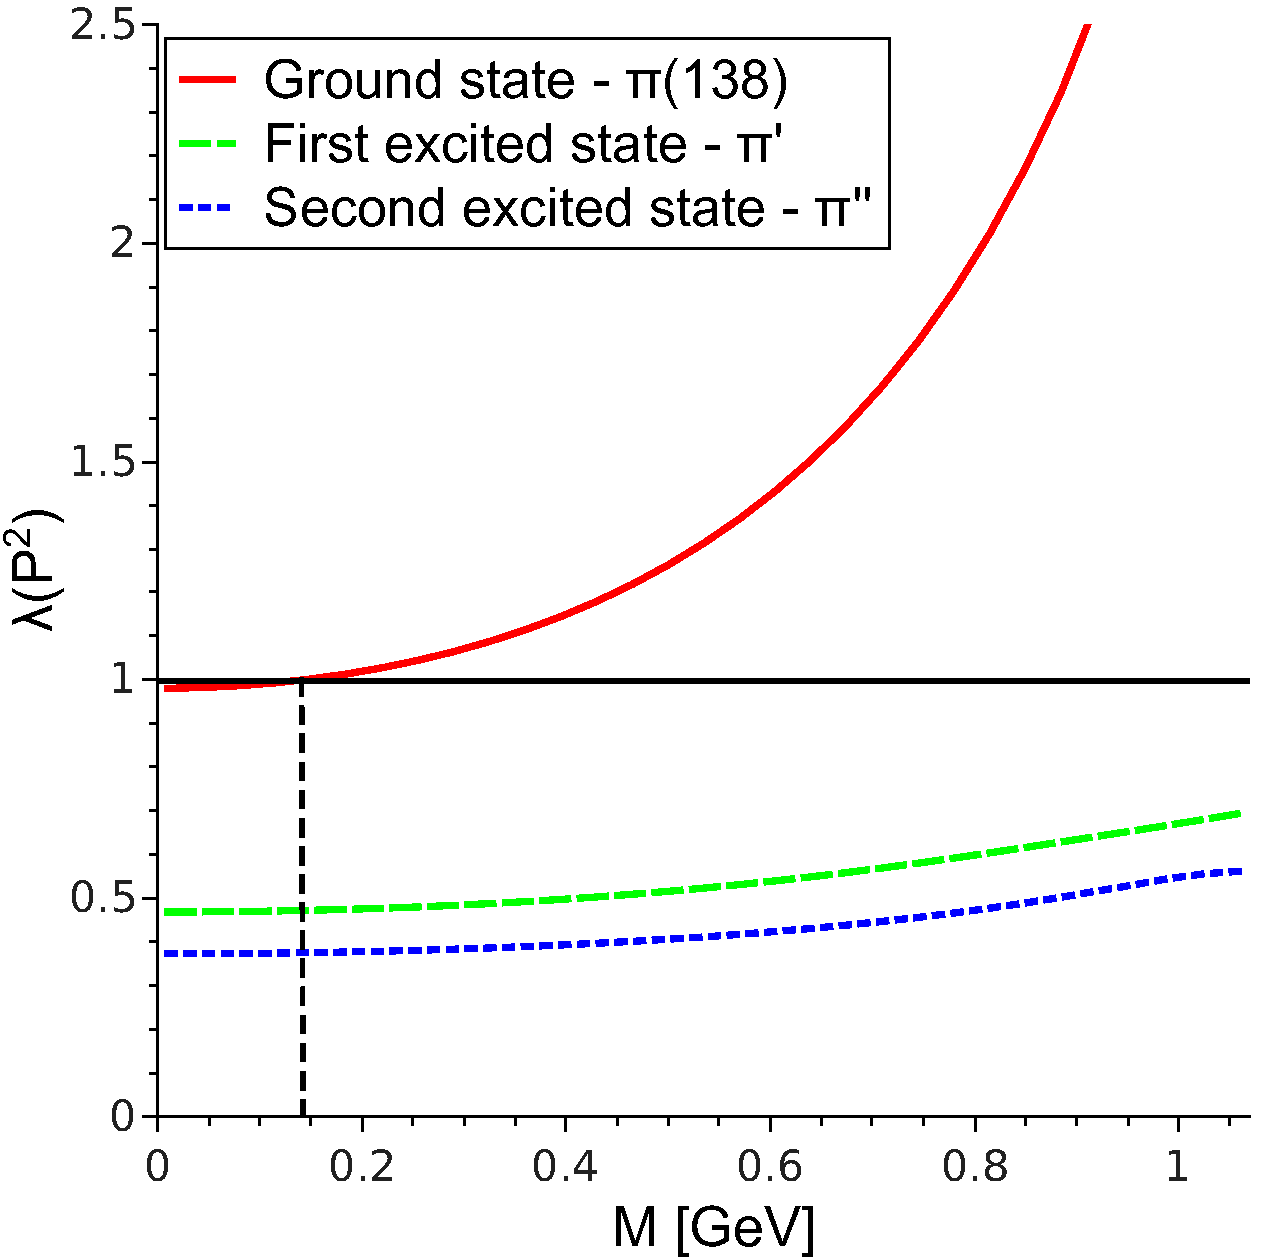
\includegraphics[width=0.49\textwidth]{figures/lambda_pseudo} 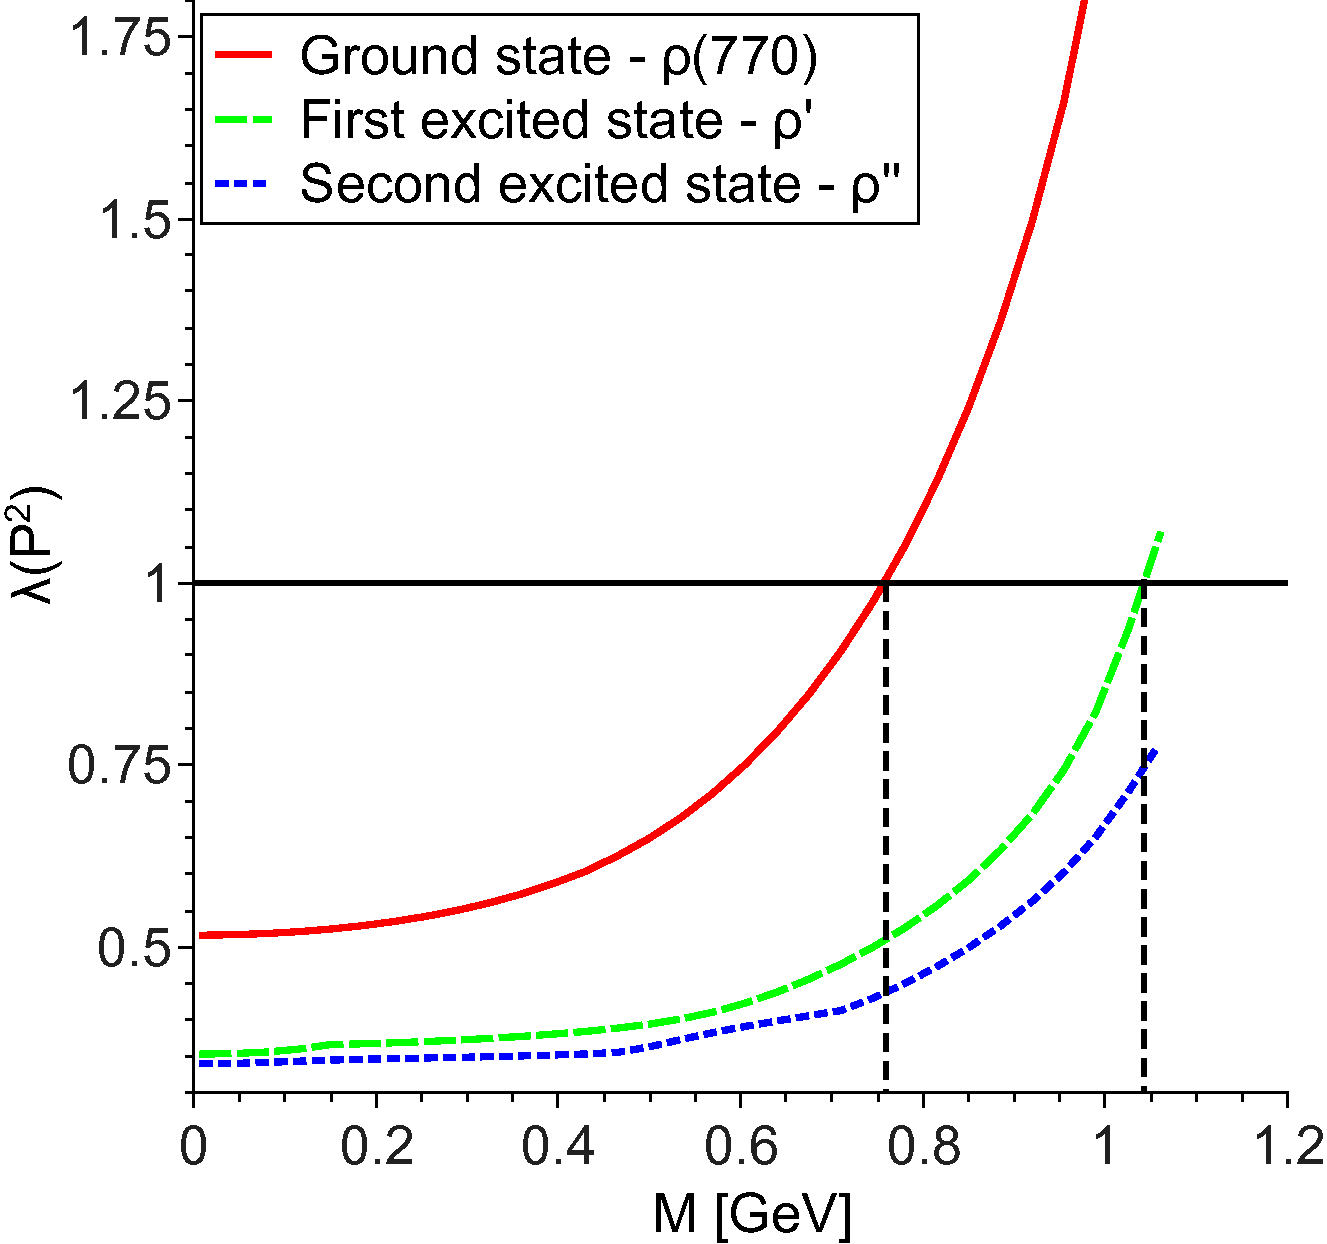
\includegraphics[width=0.49\textwidth]{figures/lambda_vector}
\caption{\footnotesize The behaviour of $\lambda$ in respect to $P^2$ for pion and rho correspondingly.}\label{fig:lambda_pseudo_vector}
\end{center}
\end{figure}
\begin{figure}[H]
\begin{center}
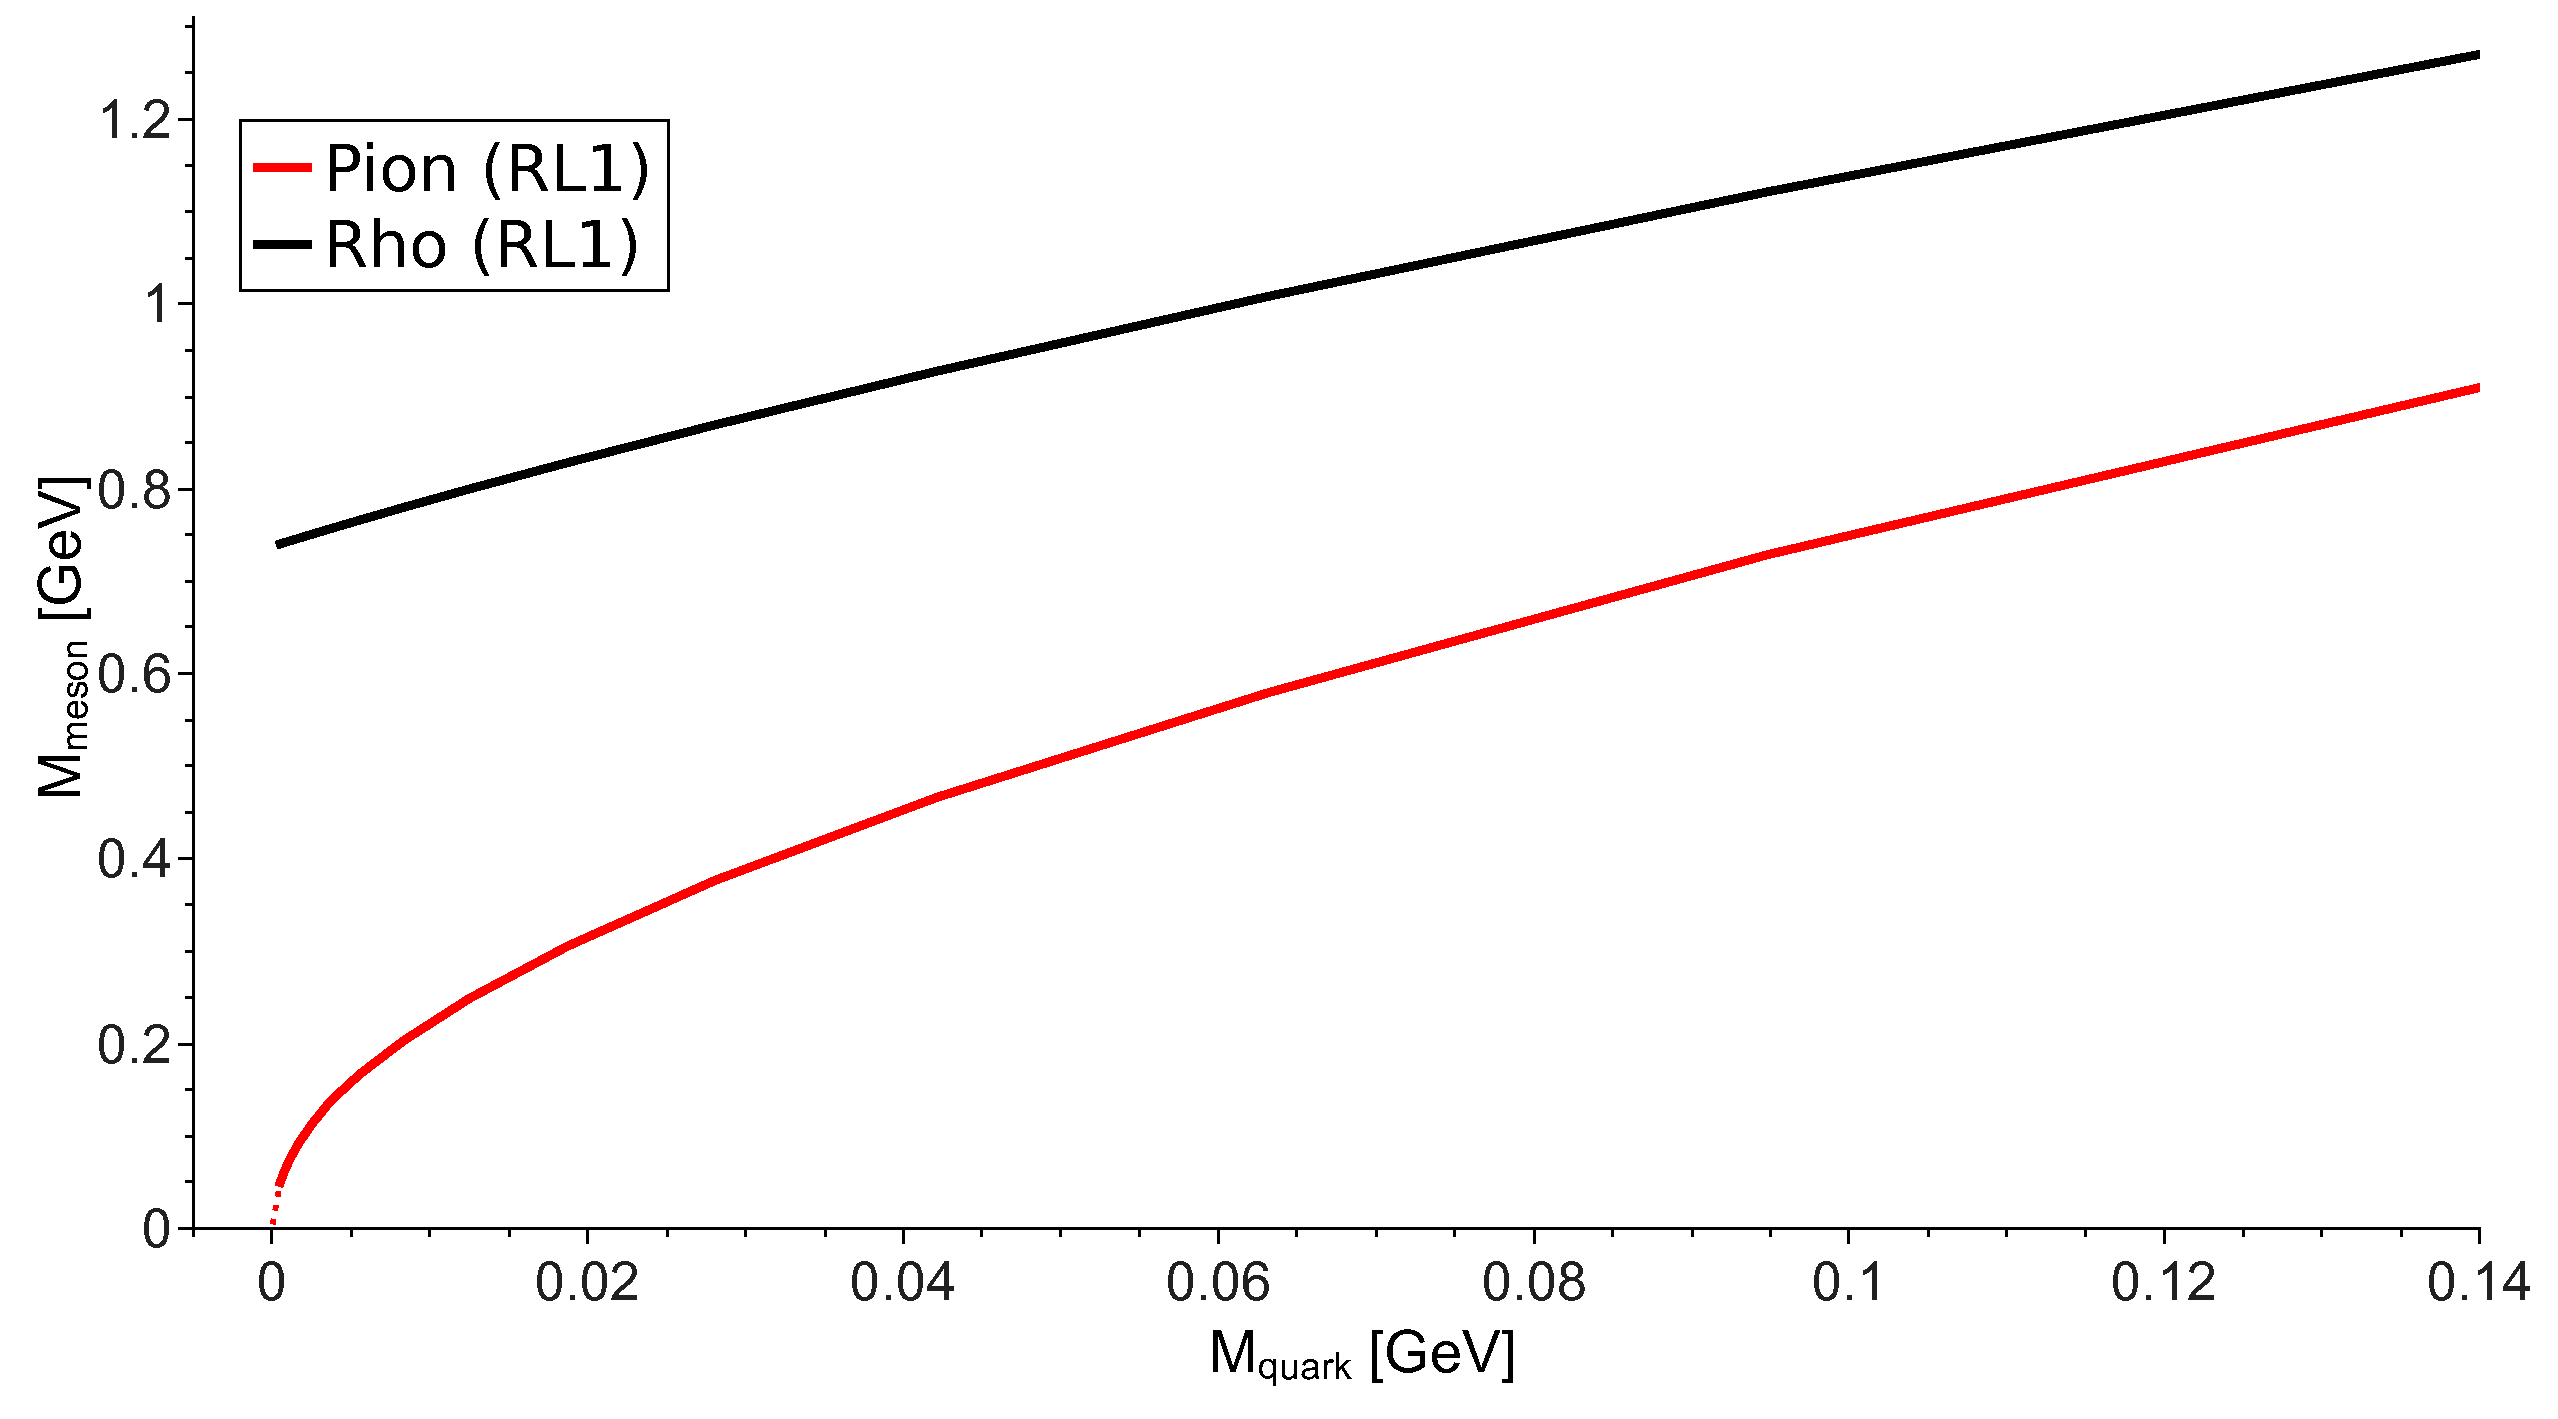
\includegraphics[width=0.99\textwidth]{figures/GMOR_RL} 
\caption{\footnotesize The pion and rho bound states masses as functions of the quark mass. GMOR square root type behaviour for the pion in the vinisity of chiral limit is indicated. }\label{fig:GMOR_RL}
\end{center}
\end{figure} 
\begin{figure}[!]
\begin{center}
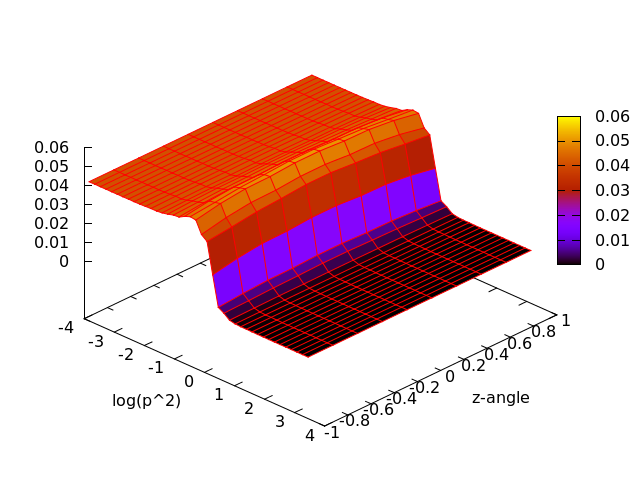
\includegraphics[width=0.80\textwidth]{figures/bsa_vector_ground} 
\caption{\footnotesize The $\gamma^\mu$ component of vector meson \BS amplitude of ground state in respect to $(p^2,z)$ dependence.}\label{fig:bsa_vector_ground}
\end{center}
\end{figure}
\begin{figure}[H]
\begin{center}
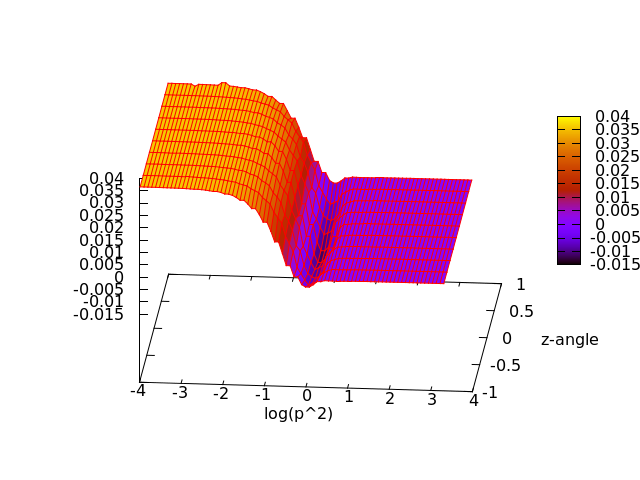
\includegraphics[width=0.80\textwidth]{figures/bsa_vector_excited} 
\caption{\footnotesize The $\gamma^\mu$ component of vector meson \BS amplitude of excited state in respect to $(p^2,z)$ dependence.}\label{fig:bsa_vector_excited}
\end{center}
\end{figure} 
The result of such calculation is a point on the graph $(\lambda(P^2),M)$, where $P^2 = - M^2$. In order to find the mass of meson bound state we search the point where the eigenvalue curve crosses the line $\lambda(P^2)=1$, as it is illustrated on Fig. \ref{fig:lambda_pseudo_vector} for $J^{PC} = 0^{-+}$ pseudoscalar channel and for $J^{PC} = 1^{--}$ vector channel. The employed single gluon rainbow-ladder truncation fulfils GMOR behaviour as it is shown on Fig. \ref{fig:GMOR_RL}. Note that our calculation is not restricted to only ground state, in principal the eigenvalue calculation gives access to the lambda curve of any excited state and the limit how high we search for the state to appear comes only from non-analytical structure of used quark propagator. \\ 

This approach is also beneficial since for every eigenvalue $\lambda$ we can obtain corresponding eigenvector $\mathcal{A}$, and therefore the meson vertex function $\Gamma^{(\mu...)}(p;P)$. As an example the first amplitude of ground state $\rho(770)$ in vector channel is given on Fig. \ref{fig:bsa_vector_ground}, together with the first amplitude of excited state $\rho^\prime$ on Fig. \ref{fig:bsa_vector_excited}. It is apparent that the BSA of excited state expose zero-crossing along the $p^2$ axis. The similar behaviour for meson wave function we can see if we consider the radial excitations within the naive quark model calculation involving Schroedinger equation with Cornell potential. This fact allows us to identify the radial excitations among obtained excited states.
%However it is not the only way to observe a bound state within meson \BSE. The another approach is to consider the off-shell versions of corresponding meson BSEs, given by Eq.(\ref{bse:BSE_inhom}) in form:
%\beqa
%	\Gamma^{(\mu...)}(p;P) = \Gamma^{(\mu...)}_{0}(p;P) + \int_k K(p,k;P)\left[ S(k_+)\Gamma^{(\mu...)}(k;P)S(k_-)\right]\;
%	\label{spectra:BSE_inhom}
%\eeqa
%
\section{Light Quark Meson Spectroscopy}
%
Firstly we consider the \textit{rainbow-ladder} ansatz, where the interaction kernel admits no mixing between states. Furthermore we work in the isospin symmetric limit using equal current quark masses $m_u=m_d=0.0037$ GeV at a renormalization scale of $\mu = 19$ GeV. Since we are in isospin symmetric limit, our calculated meson spectrum is degenerate in the isoscalar/isovector channel for $n=u,d$ quarks. The explicit numbers can be found in Table \ref{tab:results_n&s} and in Table \ref{tab:results_ns}. In Fig.~\ref{fig:spectrumnn} we display the resulting spectrum for $n\bar{n}$ mesons, and compare with the isovector channel from experiment. The input up/down quark masses are fixed such that the experimental mass of the $\pi_0$ is reproduced. The resulting ground state mass in the vector channel is also in good agreement with experiment. This is not true, however, for the scalar and axialvector states as noted frequently before, see e.g. \cite{Watson:2004kd}. Here, the deficiency of the rainbow-ladder truncation is obvious and on the 20-40 \% level. In the scalar channel there is some evidence that the lowest lying nonet may not be identified as simple quark-antiquark states, but may be better described as tetraquarks, see {\it e.g.} \cite{Jaffe:1976ig,Giacosa:2006tf,Ebert:2008id,Parganlija:2012fy,Heupel:2012ua} and Refs. therein. Therefore we compare with the $a_0(1450)$, noting that in rainbow-ladder and without potential mixing with the scalar glueball state there is no hope to reproduce the experimental value. \\

The situation is considerably better for the lowest lying tensor state \cite{Krassnigg:2010mh}, which for the upper value of the considered $\eta$-band is even on the 5 $\%$ level compared to the experimental value. While the other tensor states are again far off, at least where comparison with experiment is possible, the situation is again acceptable for the tensor meson with $J=3$ and $PC=\{--\}$. Its mass of $1528^{+71}_{-184}$~MeV compares well with both the isovector $\rho_3$ of mass $1688.8\pm2.1$~MeV (shown in the figure) and the isoscalar $\omega_3$ of mass $1667\pm4$~MeV with again a deviation on the 5 $\%$ level for the upper range of the $\eta$-band. In contrast, we find no bound state in the $J^{PC}=3^{+-}$-channel, whereas for the $J^{PC}=3^{++}$ state with mass $1510^{+81}_{-100}$~MeV there is no well established experimental counterpart.
The good agreement in states $J^{PC}=1^{--},2^{++},3^{--}$ with experiment can be explained in notions of the (pseudo)-potentials used in the quark model. In this language, what distinguishes these channels from the others is that the non-contact part of the spin-spin interaction 
is vanishing or small: for the hyperfine splitting between the pseudoscalar and vector 
\begin{figure}
\begin{center}
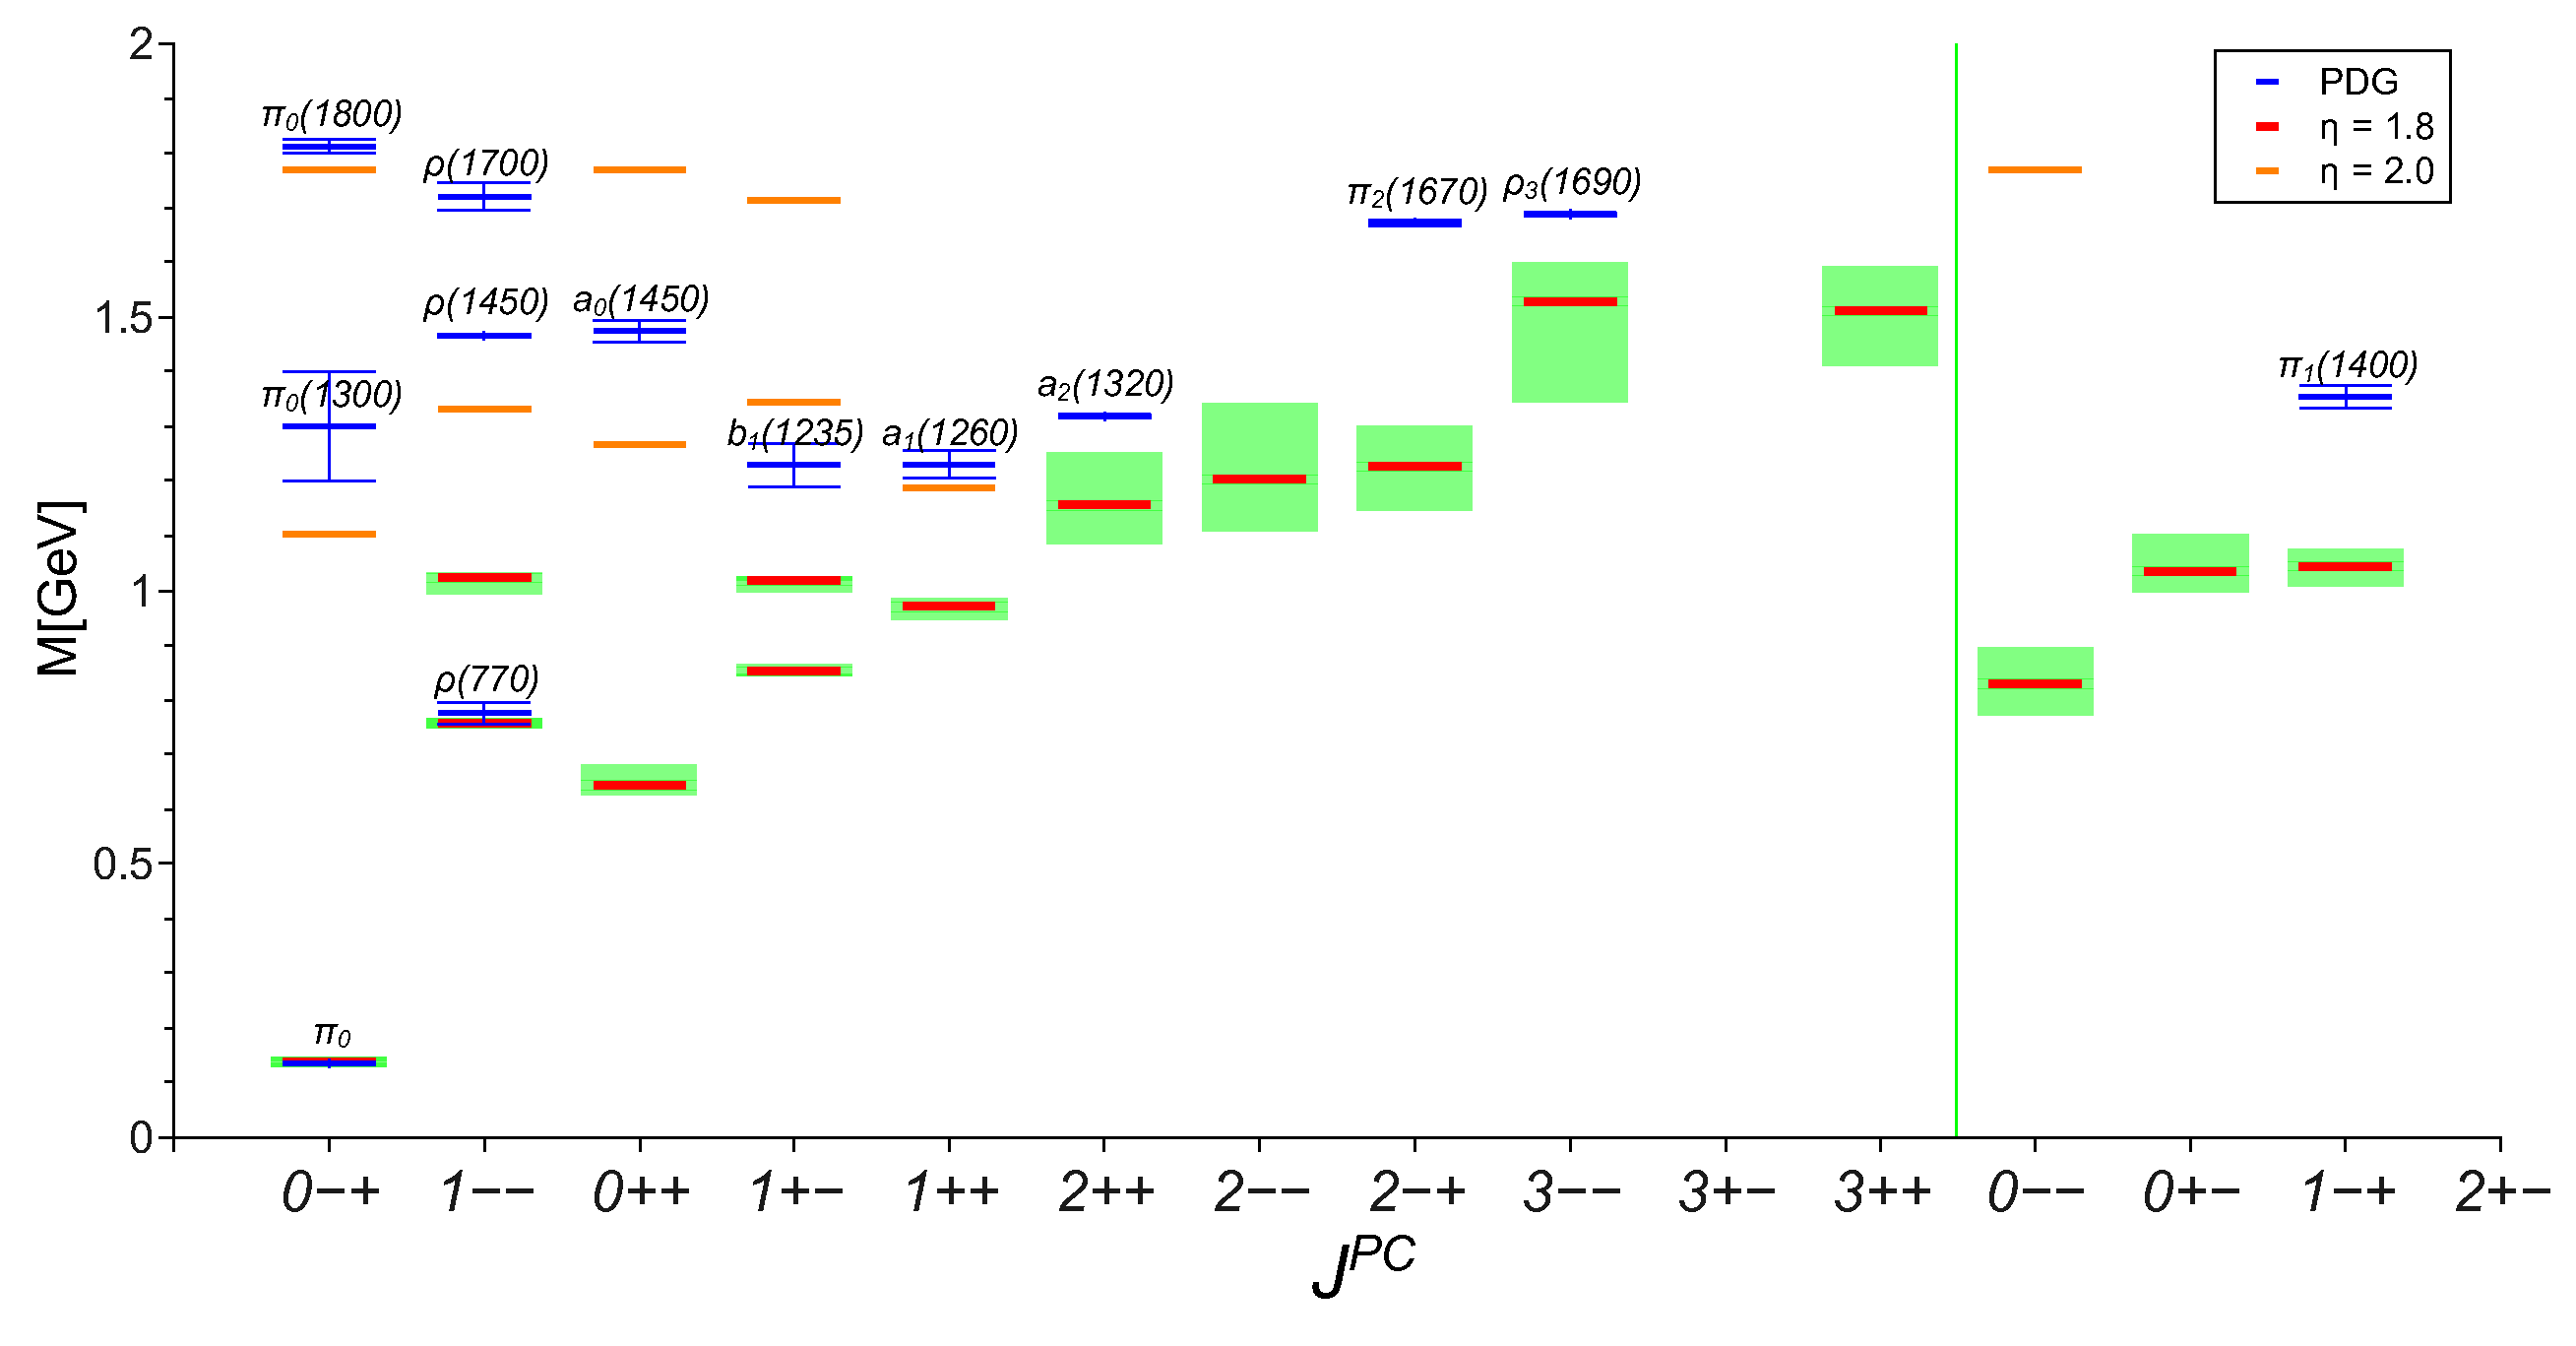
\includegraphics[width=0.999\textwidth]{figures/spectrum_nn}
\caption{\footnotesize The calculated $n\bar{n}$ spectrum, compared to the isovector mesons as measured in 
experiment. The green bands correspond to the 
variation $\eta=1.8\pm0.2$. Due to the structure of the propagator, in the case of $\eta=2.0$ more states are accessible; 
these are given by the single orange lines. The states to the right of the dividing line correspond to exotic quantum 
numbers.}\label{fig:spectrumnn}
\end{center}
\end{figure}
channels the contact part of the spin-spin interaction is dominant, whereas for the $J^{PC}=2^{++},3^{--}$
states the spin-orbit forces prevail. For all other channels considered, there are sizeable 
contributions from the tensor part of the spin-spin interaction. Since these are the channels
that are off, we conclude, that the rainbow-ladder interaction roughly reproduces the size of
the contact part of the spin-spin interaction and the spin-orbit force, but materially overestimates
the binding in the tensor part of the spin-spin interaction. 
\begin{figure*}[t]
\begin{center}
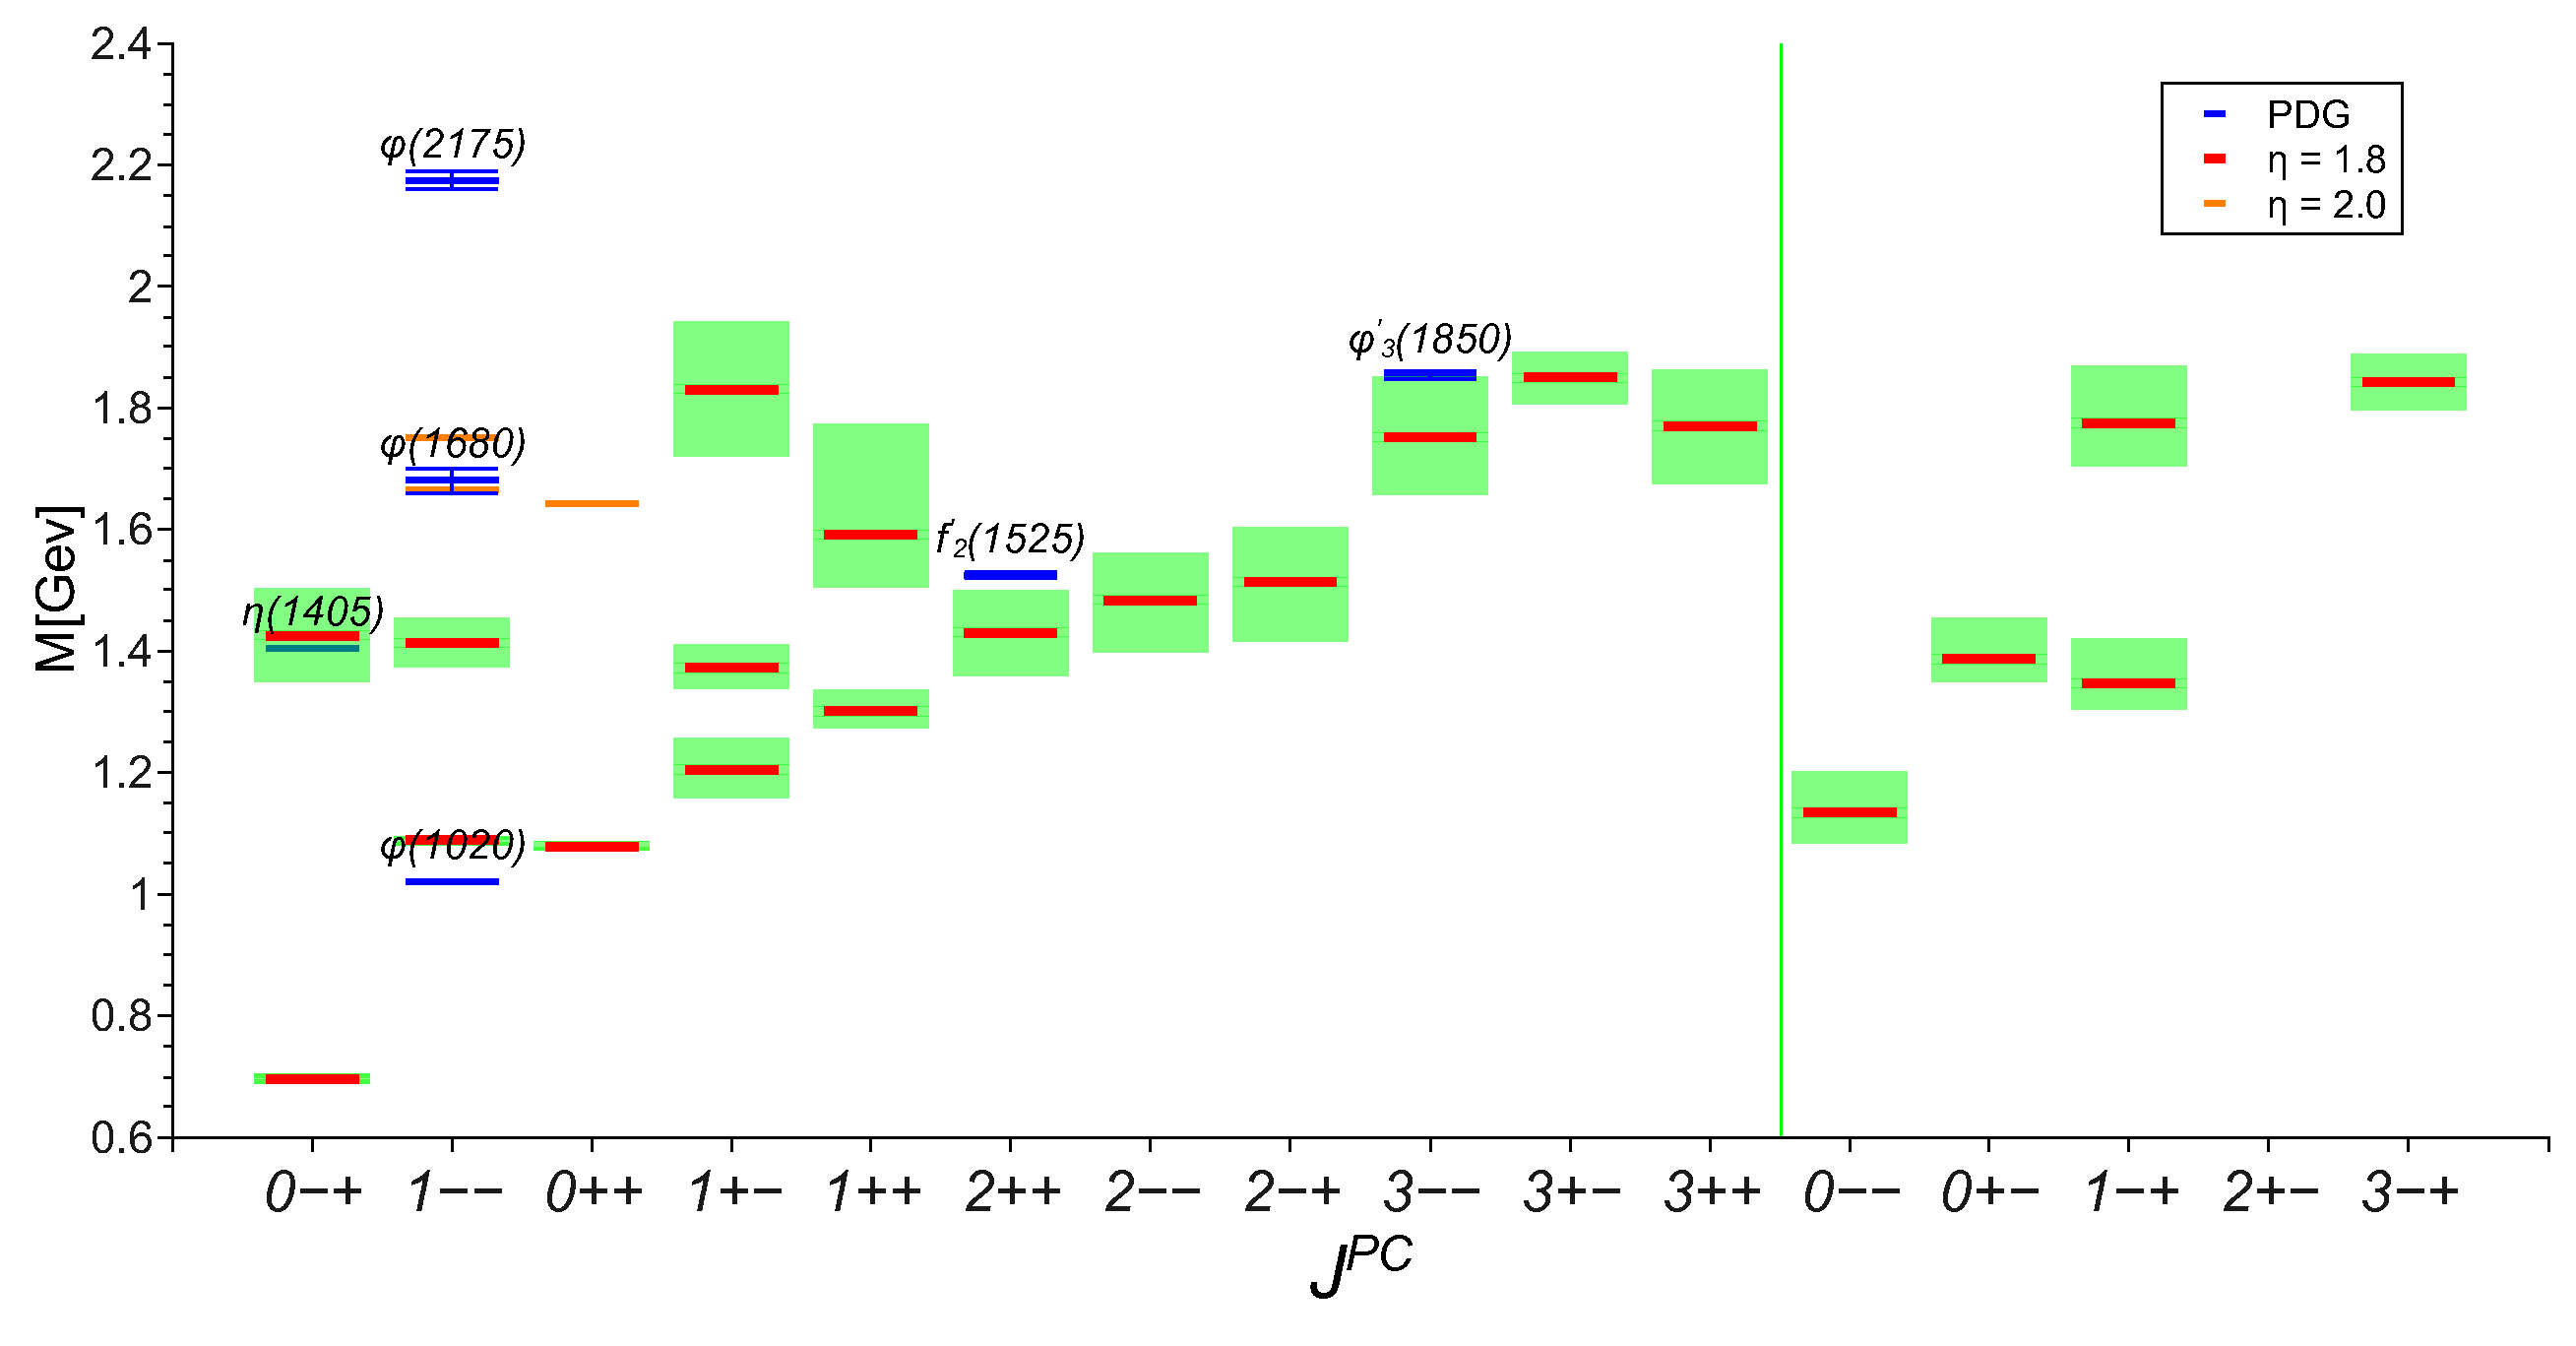
\includegraphics[width=0.999\textwidth]{figures/spectrum_ss}
\caption{ \footnotesize Calculated $s\bar{s}$ spectrum, compared to experiment. The green bands correspond to the 
variation $\eta=1.8\pm0.2$. Due to the structure of the propagator, in the case of $\eta=2.0$ more states are accessible; 
these are given by the single orange lines. The states to the right of the dividing line correspond to exotic quantum 
numbers.}\label{fig:spectrumss}
\end{center}
\end{figure*}\\

As for the exotic channels we find states for $J^{PC}=0^{--},0^{+-}$ with no experimentally established
counterpart, whereas our value for the $J^{PC}=1^{-+}$ is about 25 $\%$ lower than the $\pi_1(1400)$. The physical nature of these exotic states
is yet obscured, indicating the need to extend the effective single gloun exchange model further.
Concerning the excited states, these are in general much too low \cite{Holl:2004fr}
in agreement with the general finding for the ground states. A variation of the $\eta$-value
in general does not improve this picture; also it is noteworthy that higher excited states only
appear for very specific values of $\eta$.  \\

Next we discuss the $s\bar{s}$ spectrum displayed in Fig.~\ref{fig:spectrumss}.
Here the input value of the strange quark mass of $m_s(19 \,\mbox{GeV}) = 0.085$ GeV at the renormalization
point is determined from matching to the experimental value of the kaon mass.
First note that the pseudoscalar $s\bar{s}$-state is too light in this truncation since neither the 
effect of the $U_A(1)$ anomaly (see {\it e.g.} \cite{Alkofer:2008et} for a treatment of the anomaly
in the BSE formalism) nor flavor mixing with the $n\bar{n}$ states is considered. For the excited 
state in the pseudo-scalar channel the surprisingly excellent agreement with the $\eta(1405)$ extracted from
experiment may be accidental. In the vector channel, where mixing effects do not play a major role we
observe good agreement of our bound state mass with experiment. The same is true for the $J^{PC}=2^{++}$
and $J^{PC}=3^{--}$ channels, where the upper boundary of the $\eta$-band almost reproduces the
experimental values for the $f_2(1525)$ and the $\varphi_3(1850)$. Again, these are the channels
with dominating spin-orbit forces in the language of the potential models. In general, the pattern of
states in the $s\bar{s}$ spectrum is very similar to the one found for the $n\bar{n}$ mesons due
to the flavor independence of the underlying rainbow-ladder interaction model. 
\begin{figure*}[t]
\begin{center}
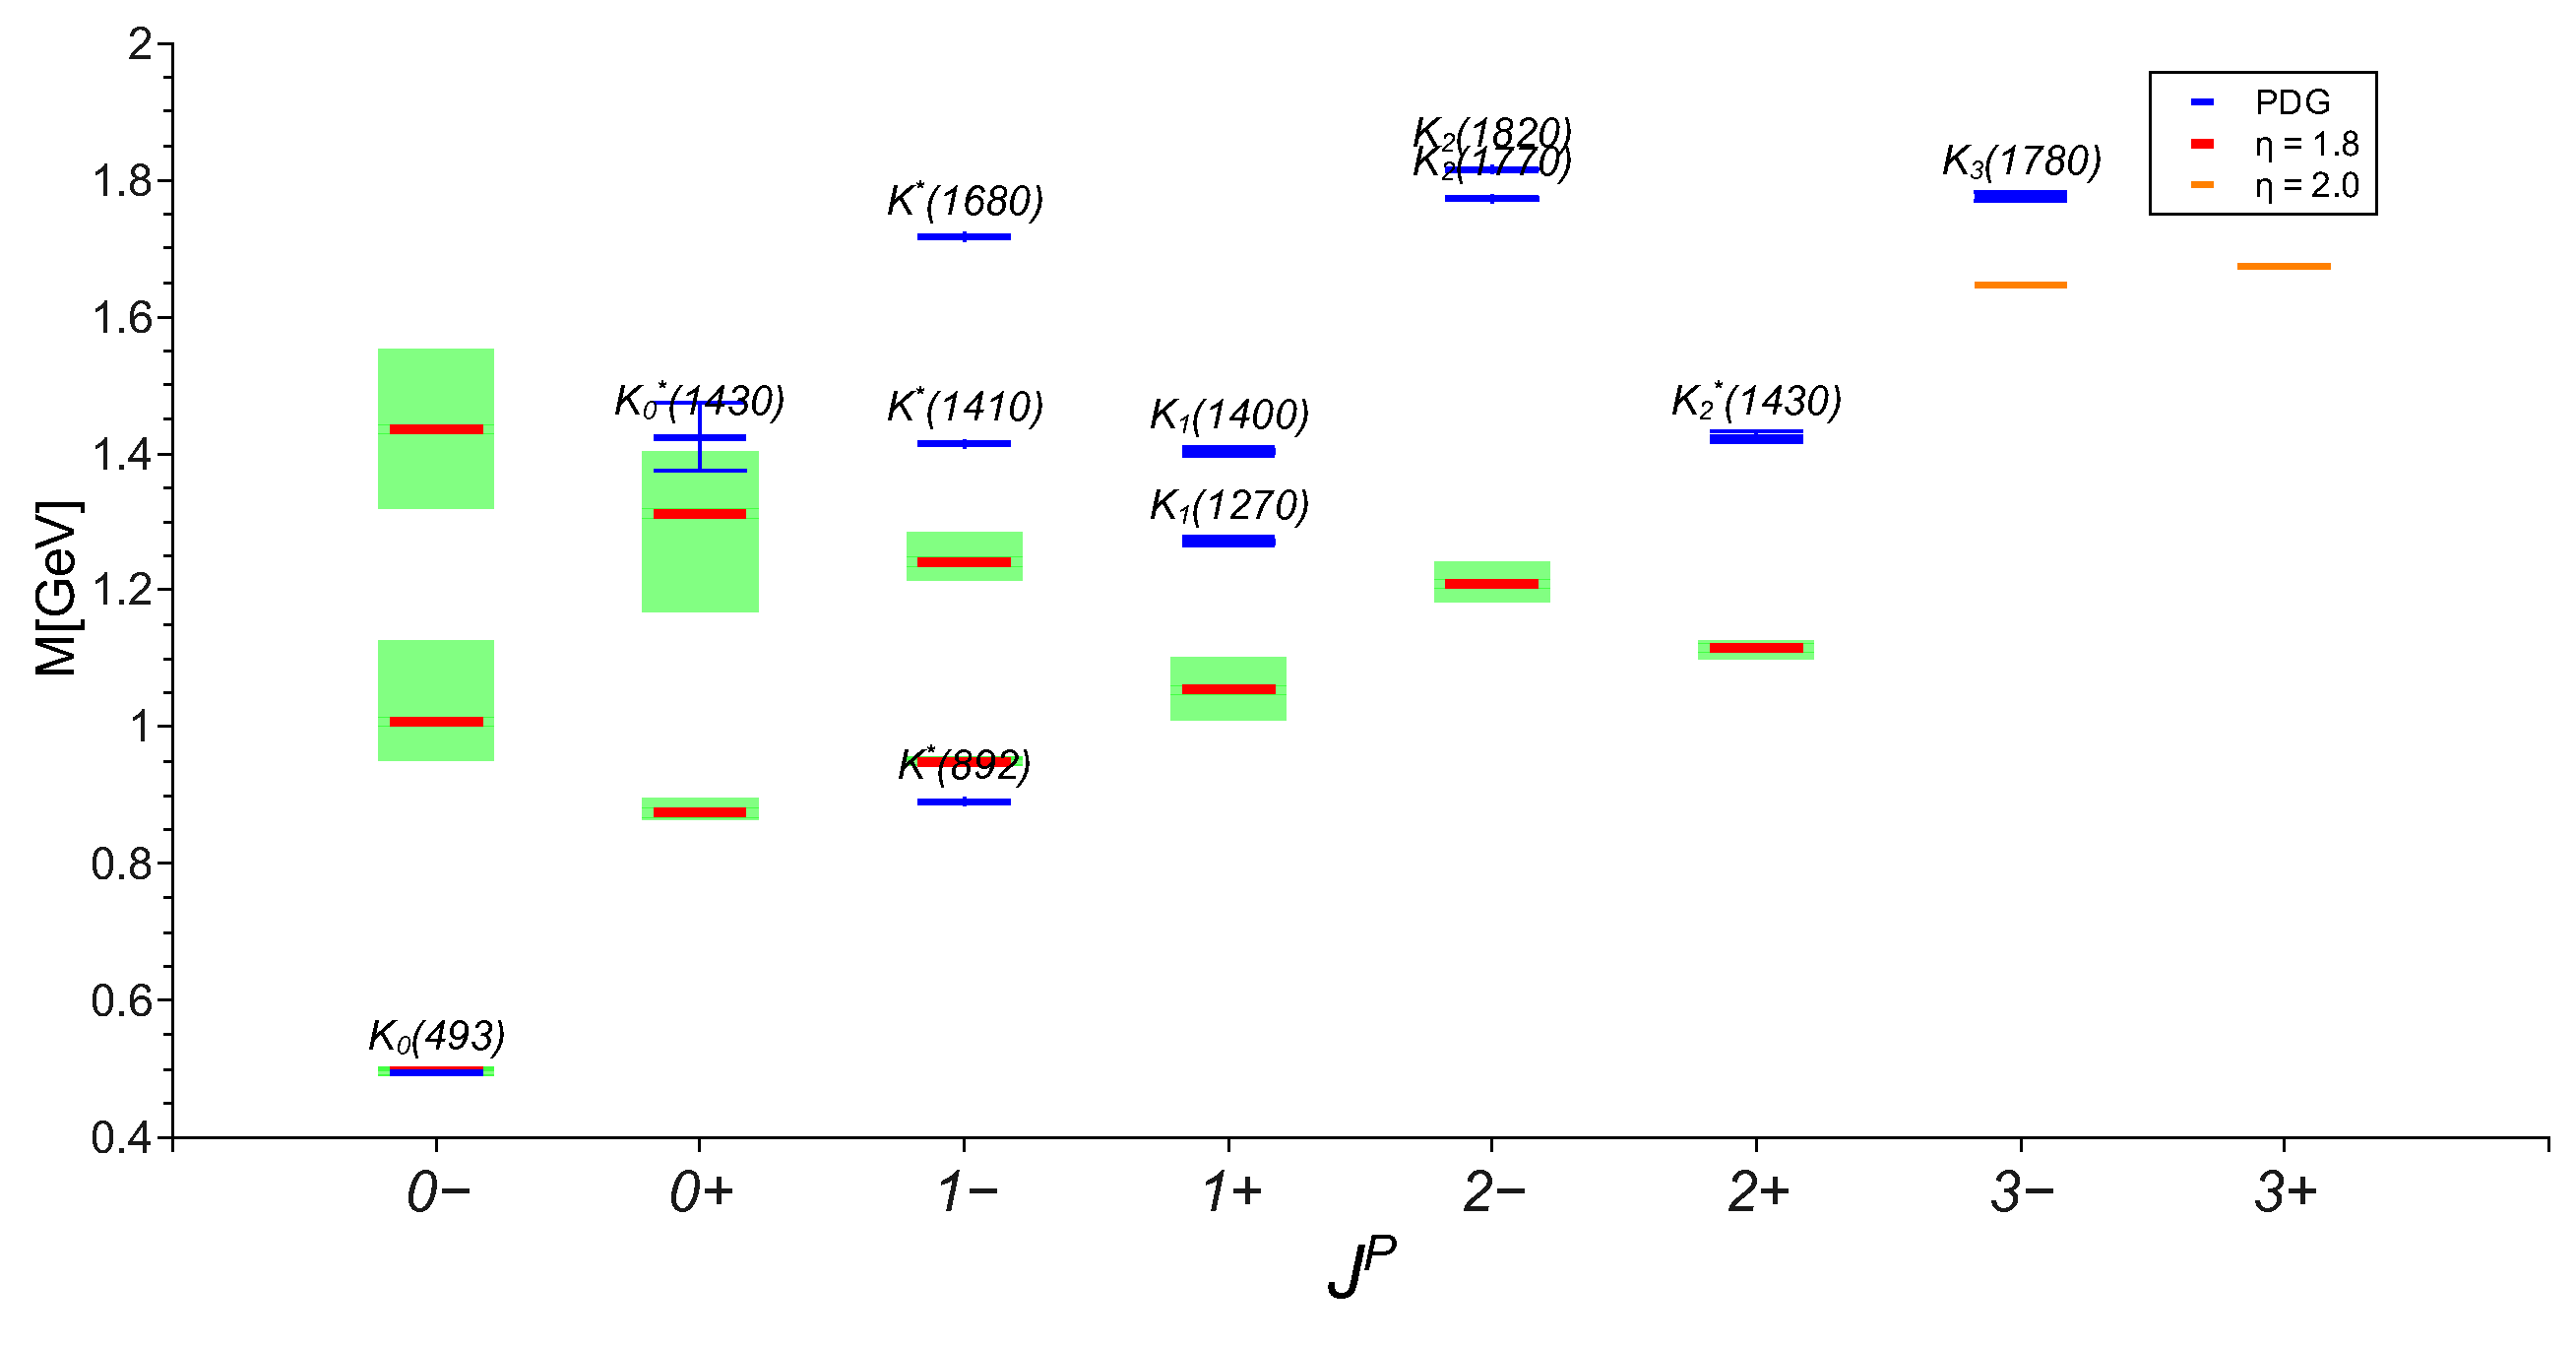
\includegraphics[width=0.999\textwidth]{figures/spectrum_ns}
\caption{\footnotesize Our calculated $n\bar{s}$ spectrum, compared to experiment. The green bands 
correspond to the variation $\eta=1.8\pm0.2$. Due to the structure of the propagator, in the case 
of $\eta=2.0$ more states are accessible; these are given by the single orange lines. The states 
to the right of the dividing line correspond to exotic quantum numbers.
 }\label{fig:spectrumns}
\end{center}
\end{figure*} \\

In the case of strange mesons, $n\bar{s}$, one is no longer able to assign either $C$ or $G$ 
parity to a state. Thus, here there are no states with explicitly exotic quantum numbers.
\begin{table*}[!th]
\renewcommand{\arraystretch}{1.3}
\begin{tabular}{c|ccc|ccc|}
\hline
\hline
                            & \multicolumn{3}{c|}{$n\bar{n}   $}                                                         & \multicolumn{3}{c|}{$s\bar{s}$}  \\
$J^{PC}$                    & $n=0$                                &   $n=1$                            &          $n=2$ & $n=0$                     &   $n=1$                   &          $n=2$    \\
\hline                                                                                                                                                                                                     
$0^{-+}$                    & $138.1^{+1.3}_{-0.6}$                &   $1103.0^\dag$                    &  $1770.1^\dag$ &  $696.3^{+2.4}_{-1.7}$    &  $1426.3_{-76.6}$         &                   \\
$0^{--}$                    & $828.8^{+66.9}_{-57.1}$              &                                    &                &  $1133.8^{+68.0}_{-50.8}$ &                           &                   \\
$0^{++}$                    & $643.6^{+17.6}_{-37.6}$              &   $1266.9^\dag$                    &  $1769.1^\dag$ &  $1079.4^{+1.7}_{-7.9}$   &  $1643.6^\dag$            &                   \\
$0^{+-}$                    & $1035.5^{+66.8}_{-38.8}$             &                                    &                &  $1386.7^{+68.8}_{-37.9}$ &                           &                   \\
\hline                                                                                                                                                                                                     
$1^{-+}$                    & $1043.9_{-37.0}$                     &                                    &                &  $1347.3^{+73.2}_{-43.7}$ &  $1870.1^{\ddag}$         &                   \\
$1^{--}$                    & $757.2^{+1.2}_{-0.6}$                & $1022.6^{+\phantom{1}9.2}_{-29.2}$ & $1331.9^\dag$  &  $1087.8^{+1.8}_{-2.2}$   &  $1413.1^{+38.8}_{-42.1}$ &   $1666.9^\dag$   \\                                                                                                                                                                       
$1^{++}$                    & $969.4^{+15.6}_{-23.9}$              & $1188.1^\dag$                      &                &  $1301.0^{+34.7}_{-28.5}$ &  $1591.9^{+181.2}$        &                   \\
$1^{+-}$                    & $852.1^{+13.6}_{-\phantom{1}5.2}$    & $1017.4^{+\phantom{1}0.6}_{-21.4}$ & $1345.2^\dag$  &  $1205.1^{+51.8}_{-46.6}$ &  $1372.0^{+34.4}_{-39.5}$ &   $1831.6^\dag$   \\
\hline                                                                                                                                                                                                     
$2^{-+}$                    & $1226.5^{+73.9}_{-80.0}$             &                                    &                &  $1513.5^{+90.5}_{-85.0}$ &                           &                   \\
$2^{--}$                    & $1202.6^{+140.0}_{-\phantom{1}94.3}$ &                                    &                &  $1484.7^{+76.0}_{-86.0}$ &                           &                   \\
$2^{++}$                    & $1154.8^{+96.5}_{-69.3}$             &                                    &                &  $1431.4^{+72.4}_{-69.3}$ &                           &                   \\
$2^{+-}$                    &                                      &                                    &                &                           &                           &                   \\
\hline                                                                                                                                                                                                     
$3^{-+}$                    &                                      &                                    &                &  $1842.5_{-46.6}$         &                           &                   \\
$3^{--}$                    & $1528.3^{+\phantom{1}71.2}_{-184.2}$ &                                    &                &  $1751.7^{+99.2}_{-94.3}$ &                           &                   \\
$3^{++}$                    & $1510.5^{+\phantom{1}81.6}_{-100.3}$ &                                    &                &  $1770.9^{+91.4}_{-96.1}$ &                           &                   \\
$3^{+-}$                    &  								   		&                                    &                &  $1849.4_{-43.6}$ 		   &                      	     &           			\\                                                                                                                                                                      
\hline
\hline
\end{tabular}
\caption{Mass spectrum in MeV for isospin degenerate $n\bar{n}$ and isoscalar $s\bar{s}$ bound-states. The rainbow-ladder result corresponds to $\eta=1.8\pm0.2$, with the 
superscript ${}^\dag$ (${}^\ddag$) indicating $\eta=2.0$ ($\eta=1.6$) only.}\label{tab:results_n&s}
\end{table*}
The spectrum, as calculated within the rainbow-ladder approximation, is given in Fig.~\ref{fig:spectrumns}. 
As already mentioned above, the strange quark mass is chosen such that the calculated $K^{0,\pm}$ 
is in agreement in experiment; the remaining spectrum is a result of the model.
While the vector ground state is in reasonable agreement with experiment, the remaining spectrum 
does not fare so well (as in the unflavored case).
\begin{table*}
\centering
\renewcommand{\arraystretch}{1.3}
\begin{tabular}{c|ccc|}
\hline
\hline
          				     & \multicolumn{3}{c|}{$n\bar{s}$}  \\
$J^P   $&  $n=0$    &$n=1$  & $n=2$ \\
\hline                                                                                                                                                                                                     
{$0^-$}       &   { $496.6^{+5.3}_{-0.9}$} &  {$1007.6^{+118.3}_{-\phantom{1}57.0}$ } & {$1435.9$} \\                                                                                                                                                                        
{$0^+$}       &  { $874.5^{+10.0}_{-22.2}$ } &  {$1312.5^{+\phantom{1}90.3}_{-143.8}$} &  \\                                                                                                                                                                        
\hline                                                                                                                                                                                                     
{$1^-$}       &   {$ 950.1^{+5.5}_{-1.6}$} &  {$1241.6^{+43.5}_{-27.9}$ } &  \\                                                                                                                                                                  
{$1^+$}       & {$1054.1^{+48.7}_{-44.8}$} &   &  \\
\hline                                                                                                                                                                                                     
{$2^-$}       &  { $1116.2^{+10.9}_{-17.2}$ } &   &  \\
{$2^+$}       &  {$1209.4^{+32.3}_{-26.6}$} &   &  \\
\hline                                                                                                                                                                                                     
{$3^-$}       & { $1646.9^\dag$ }  &   &  \\
{$3^+$}       & { $1673.4^\dag$  } &   &  \\                                                                                                                                                                  
\hline
\hline
\end{tabular}
\caption{Mass spectrum in MeV for $I=1/2$ $n\bar{s}$ bound-states. The rainbow-ladder result corresponds to $\eta=1.8\pm0.2$, with the 
superscript ${}^\dag$ (${}^\ddag$) indicating $\eta=2.0$ ($\eta=1.6$) only.}\label{tab:results_ns}
\end{table*}
Along with the usual $J=1$ and $J=2$ mesons, we find two states with $J=3$, one with positive 
and one with negative parity. For the latter, we have a mass of $1646.9$ (found for $\eta=2.0$ only) 
which compares well with the experimentally known $K_3^\star$ whose mass $1776\pm7$ is within $10\%$. 
The positive parity state is similar in mass, $1673.4$, but the $K_3$ has not been seen in 
experiment. The results strongly indicate that the $n\bar{s}$ system should be investigated in a beyond rainbow-ladder 
approximation, in order to find stronger agreement for the majority of low-lying states. 

\section{Heavy Quark Meson Spectroscopy}
\subsection*{Charmonia}
\label{sec:charm}
%
%
%
%
%
%
We approach the study of heavy quark 2-body systems within rainbow-ladder Truncation using the vanilla Maris-Tandy interaction,
i.e. we keep the scale $\Lambda=0.72$ from the light meson sector and
explore the dependence of the spectrum on $\eta$.

Since $J^{PC}=1^{--},2^{++},3^{--}$ states are well represented in the vanilla
Maris-Tandy (MT) interaction in the light meson sector, we first concentrate
on the ground and first excited states in the $1^{--}$ and $2^{++}$-channels
and explore the variation of the corresponding masses with the charm quark
mass and the $\eta$-parameter in the MT-interaction. We obtained good
agreement with experiment using a charm quark mass of 
$m(19 \,\mbox{GeV}) = 0.870 \,\mbox{GeV}$ and a value $\eta=1.157$.
\begin{figure*}[h]
  \begin{center}
  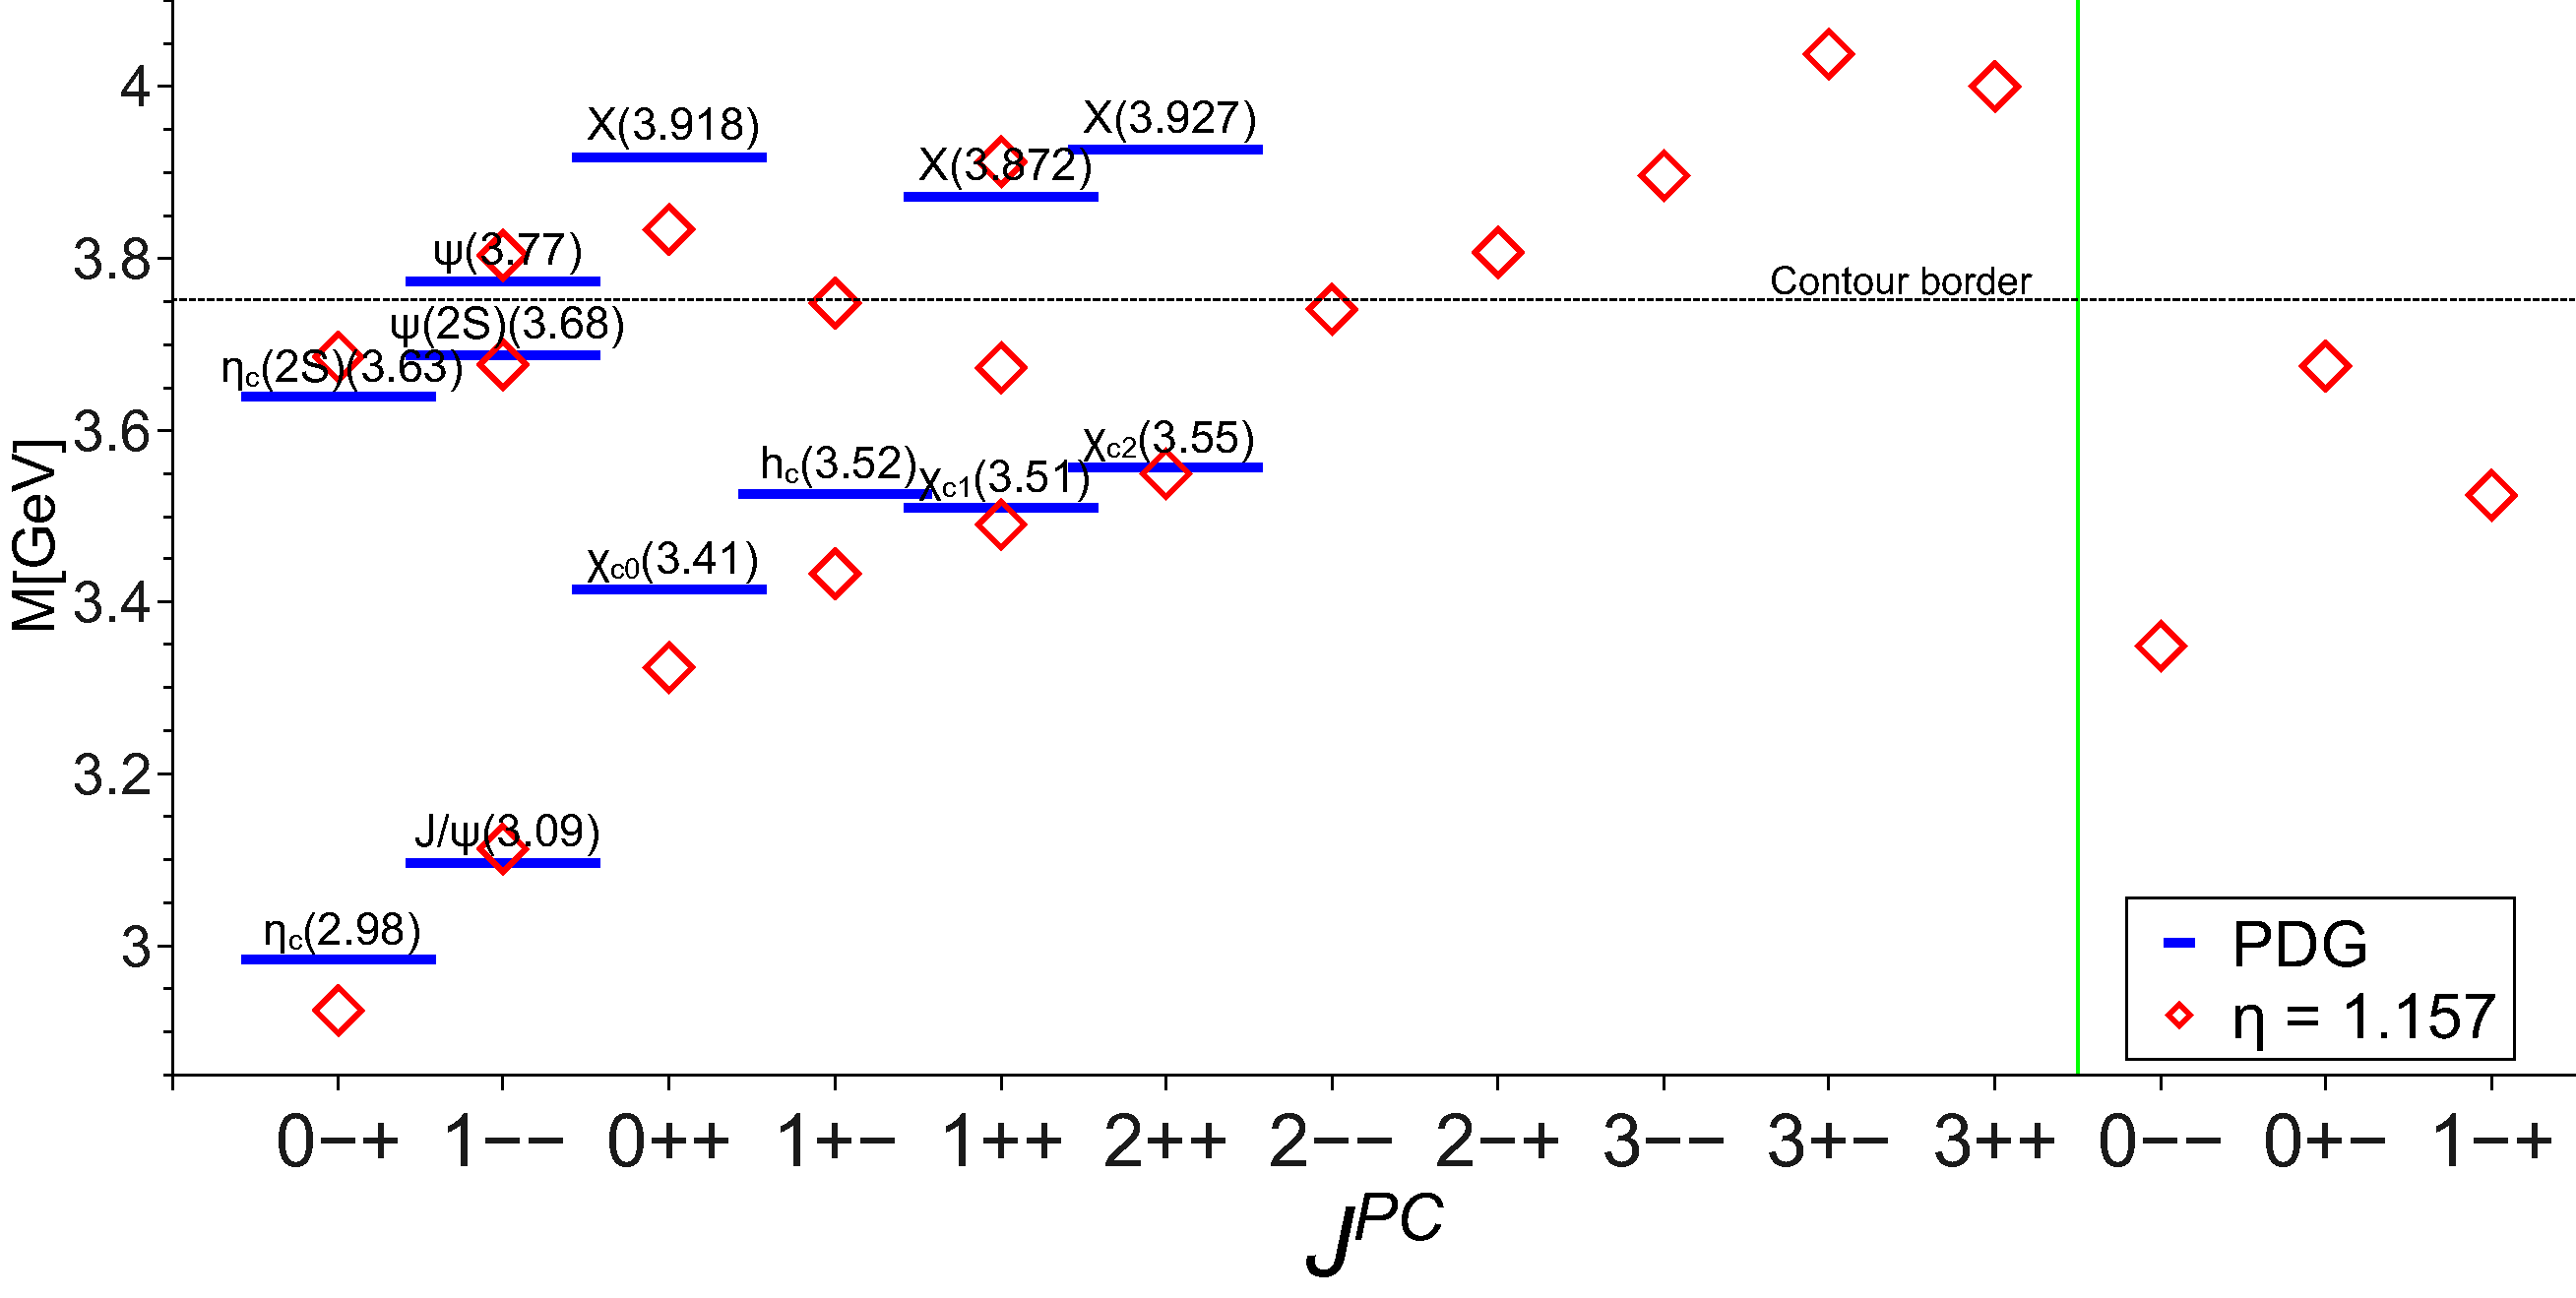
\includegraphics[width=0.999\textwidth]{figures/spectrum_cc}
  \caption{Spectrum of ground and excited charmonium states.}
  \label{fig:charm}
  \end{center}
\end{figure*}
Our results for all presently available channels are shown in Fig.~\ref{fig:charm},
the explicit values are all collected in Table. \ref{tab:results_heavy}.
Since we have fixed the two input parameters $\eta,m_{charm}$ with the $J/\Psi$ and $X_{c2}$ ground 
state, all other states can be viewed as model predictions. In the pseudoscalar channel
we find a mass of the $\eta_c$ which is slightly too low, but still within 3 \% of 
the experimental value. In the language of potential models, this may indicate an 
overestimation of the spin-spin contact term in the effective interaction. Very good 
agreement with experiment is obtained for the ground state in the $1_{++}$-channel, 
whereas the masses of the scalar $0^{++}$ and the axialvector $1^{+-}$ ground states are further 
off but still within five percent of the experimental value. Similar results have
been obtained already in Ref.~\cite{Blank:2011ha,Hilger:2014nma}. As we already observed in the light quark sector, that the rainbow-ladder interaction
is well suited to reproduce states in the sequence $1^{--}, 2^{++}, 3^{--},...$. We therefore expect our 
prediction for the mass of the $3^{--}$-state charmonium of 
%
\begin{align}
%
  m_{3^{--}}= 3.896 \,\mbox{GeV}
%
\end{align}
%
to be accurate with an error below 1~\% due to uncertainties in the interaction.
Since this state is a ground state still close to the boundary of calculable states 
(the dashed line in the plot) it is not subject to a large extrapolation error. We 
therefore expect our prediction for the mass of this state to be quite robust, with 
an overall error on the 3~\% level. Within errors, this agrees with the quark model 
prediction \cite{Ebert:2011jc} and the lattice QCD results \cite{Bali:2011rd,Liu:2012ze}.
For the other tensor ground states with $J=2$ and $J=3$ we expect much less accurate 
predictions, perhaps on the 5-10~\% level. \\ 

For the excited states we observe very good agreement in the vector channel: our
value for the mass of the $\Psi(2S)$ is very close to the experimental one, and even
the next radial excitation is nicely represented. In the pseudoscalar channel the 
splitting between the ground and the excited state is slightly too large, making the 
agreement of the $(2S)$-state with experiment even better than for the ground state
$\eta_c$. It is interesting to observe that the resulting fine structure splitting of 
the ground and excited states show a qualitatively difference when compared with 
experiment: whereas the ground state splitting is too large the splitting in the 
excited state is too low. Such an uncorrelated behaviour of the two splittings has
also been observed in lattice QCD \cite{Bali:2011rd}. \\

In the `good' tensor channel $2^{++}$ potential excited states like
the $X(3927)$ are not reproduced in our framework. There is a considerable uncertainly 
due to the extrapolation procedure needed in this mass region, which is enhanced for
excited states. Taking our result at face value, however, the current model would disregard 
the notion of the $X(3927)$ to be an ordinary meson state. \\

From an experimental point of view, the $1^{++}$-channel is perhaps the most interesting
one. There the famous $X(3872)$-state awaits its identification as a meson-molecule,
a tetraquark, or an ordinary quark-antiquark bound state. The literature on this
subject is enormous, therefore we point the reader only to Ref.~\cite{Bodwin:2013nua} 
for a first overview. The interesting question in this context is, whether a description
on a quark-antiquark basis is possible at all for the $X(3872)$. In the present
rainbow-ladder model we find an excited state in the $1^{++}$-channel at 
$m = 3672 \,\mbox{MeV}$ that cannot be accounted for by experiment. A second excitation 
is found at $m = 3912 \,\mbox{MeV}$, close to the quark model prediction for the first
excited state. In principle, it could be that the lower state of the two is spurious.
However, since we find no trace in our numerics that this is the case we disregard this
notion for the moment. It follows then, that the present form of the rainbow-ladder 
interaction is not sufficient to describe the splitting between ground and excited states
in this channel. A similar conclusion may be drawn for the other axialvector channel.
We therefore expect sizeable corrections when interactions beyond the 
rainbow-ladder approximation are taken into account. 

\subsection*{Bottomonia}\label{sec:bottom}
Our results for the spectrum of bottomonia are shown in Fig.~\ref{fig:bottom}. Compared to
the charmonium spectrum in Fig.~\ref{fig:charm} we had to change the shape of the interaction
by adjusting the $\eta$-parameter from $\eta=1.157$ for the charm-case to $\eta=1.357$ 
for the bottom quarks. This reflects part of the underlying flavour dependence of the quark-gluon 
interaction as noted in Ref.~\cite{Williams:2014iea}. Our corresponding mass of the bottom quark
is $m(19 \,\mbox{GeV})=3.790 \,\mbox{GeV}$. The resulting spectrum of ground and excited states, 
however, has similar features when compared with experimental values as the charmonium one. 
Once again, the $0^{-+}$, $1^{--}$ and $2^{++}$ ground states are well represented. The necessary
extrapolation needed for the $2^{++}$ is still under control, since the state is not too far above
the limit where everything can be calculated (the dashed line in the plot). Surprisingly good is
also the negative parity tensor state, although the extrapolation procedure in this
mass region must be considered with a little more caution. \\

Provided the good agreement in the $2^{--}$-channel can be seen as an indication that 
extrapolation even in this mass region works well, we can regard the masses of the 
further tensor states with $J=2$ and $J=3$ as solid predictions. For $3^{--}$ bottomonium bound state we found:
\begin{align}
%
  m_{3^{--}}= 10.232 \,\mbox{GeV}
%
\end{align}
Compared to the quark-model predictions of \cite{Ebert:2011jc}
we find only slight deviations of the order of 30-70 MeV for the $2^{-+}$ and the states 
with $J=3$.
%
\begin{figure*}[t]
  \begin{center}
    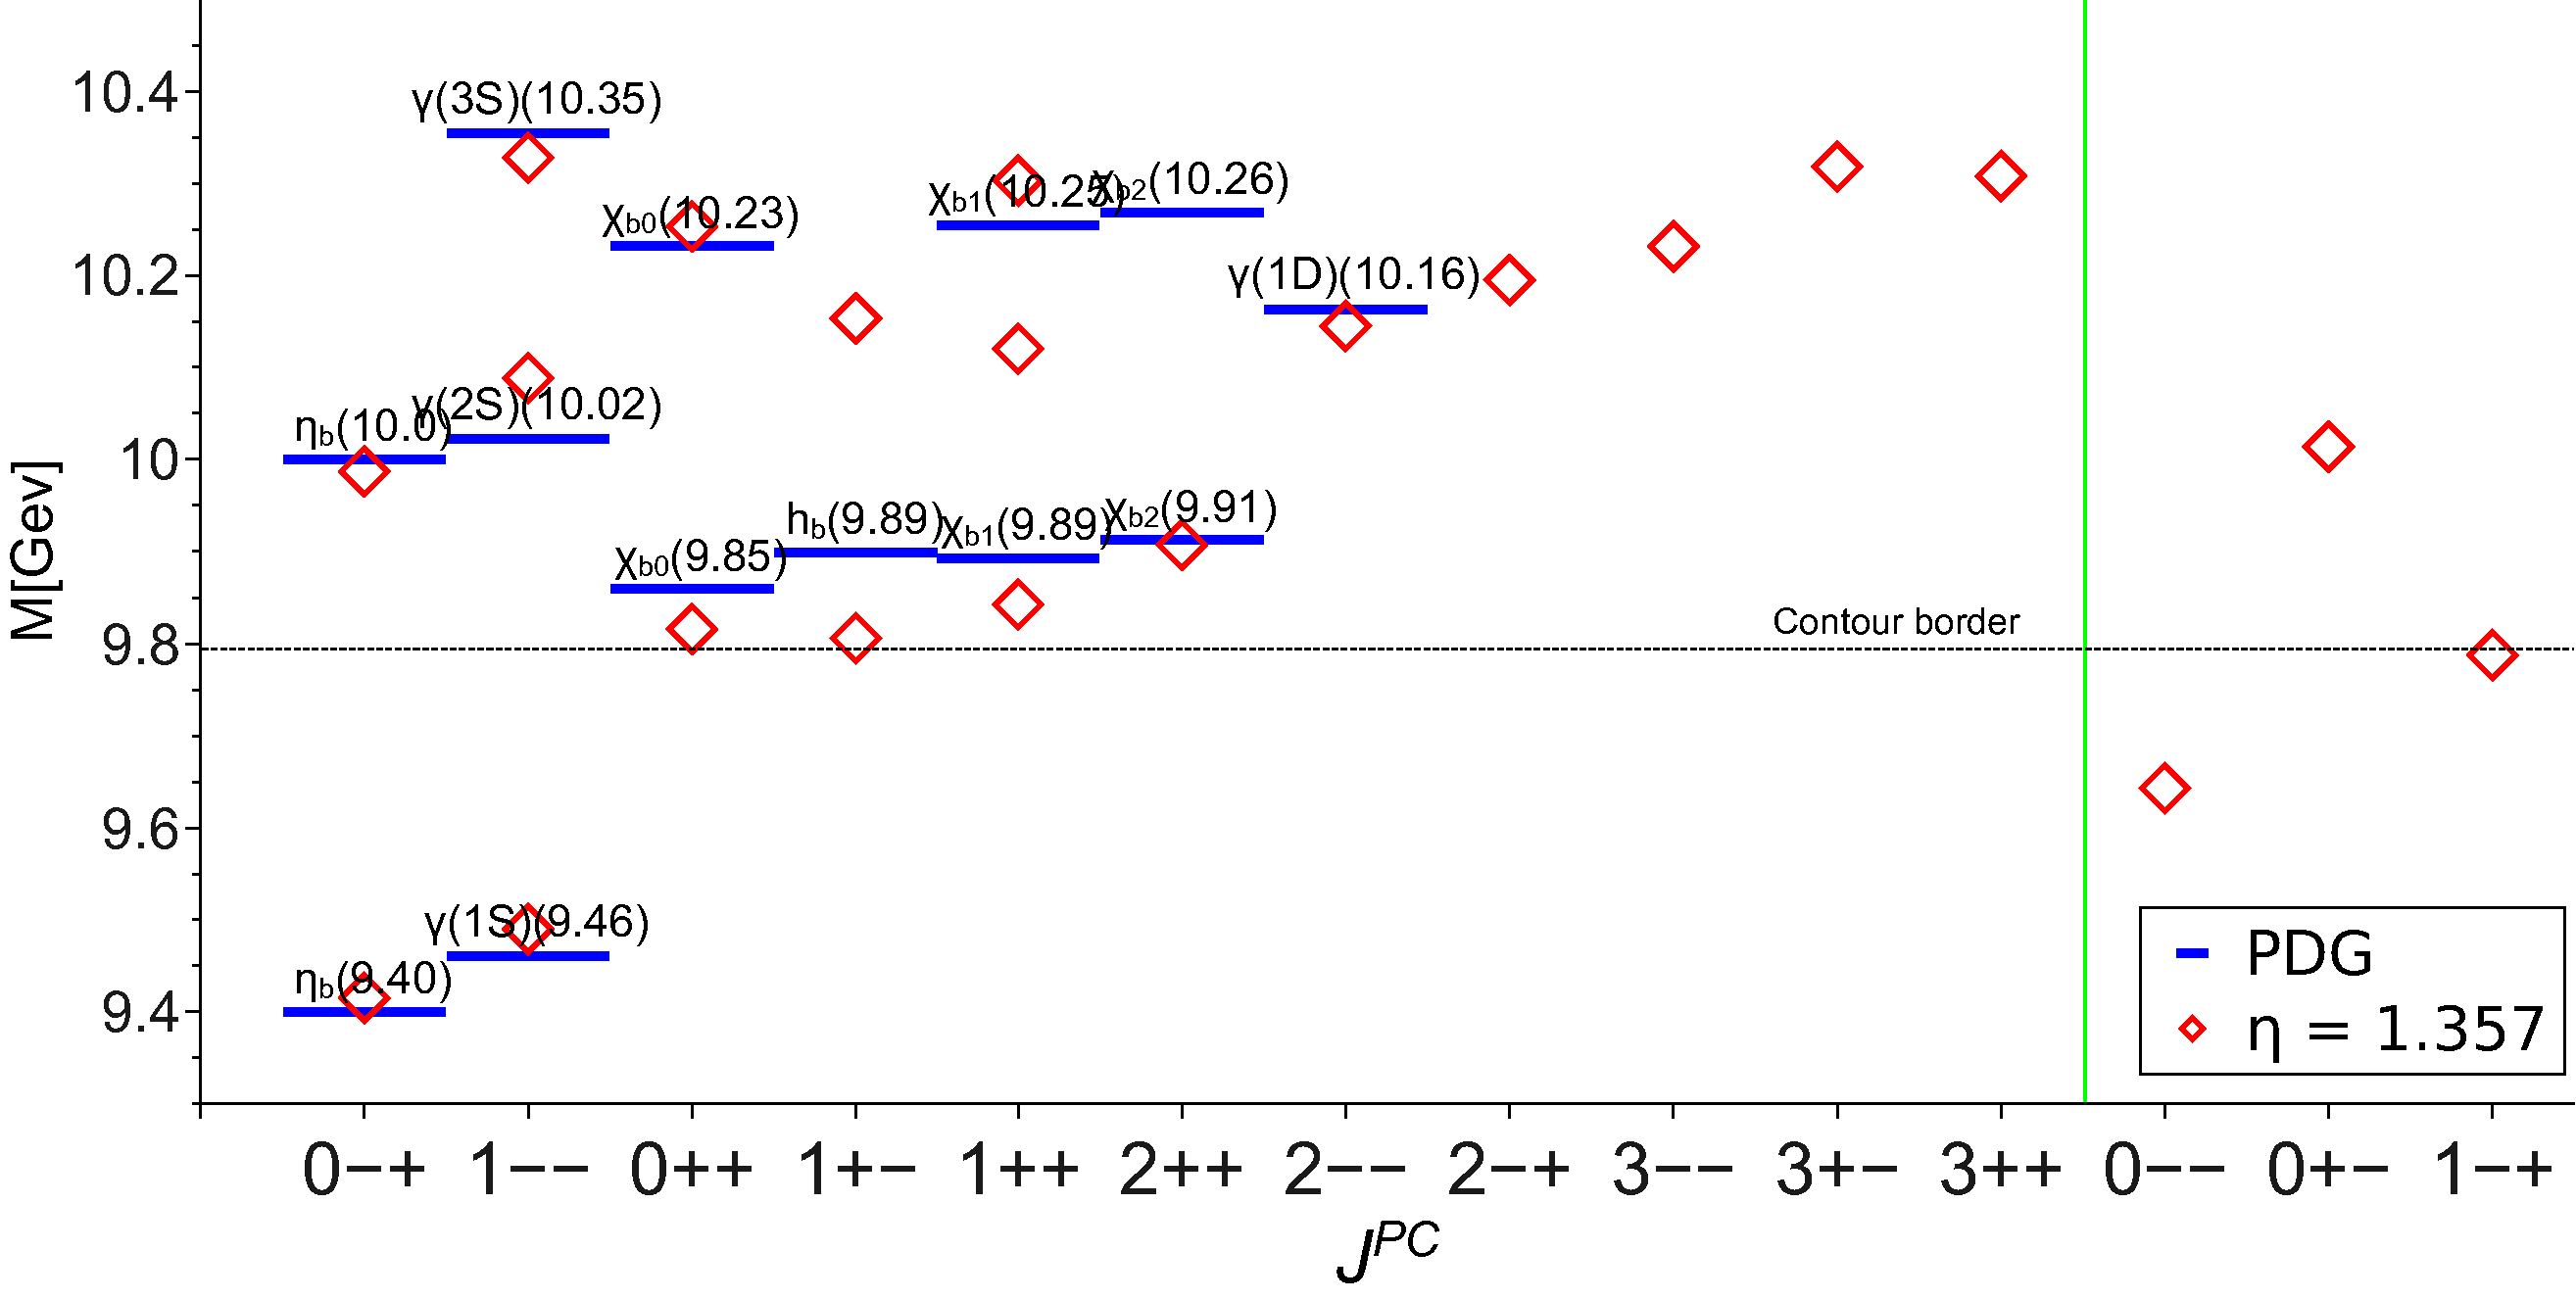
\includegraphics[width=0.999\textwidth]{figures/spectrum_bb}
    \caption{Spectrum of ground and excited bottomonium states.}\label{fig:bottom}
  \end{center}
\end{figure*}
%
In contrast to the charm-case, the lowest lying excited states in the bottomonium spectrum are
already in a mass region where we need to extrapolate the eigenvalue of the BSE, as discussed
above. Nevertheless, the results are surprisingly good and comparable with the corresponding ones in the charmonium spectrum, where much less
extrapolation was needed. The first excited states in the pseudoscalar, vector and even the
scalar channel are quite accurate and even the $\Psi(3S)$ works reasonably well. In the $1^{++}$-channel
we encounter the same problem as in the charmonium spectrum, there is a first excited state 
with a much too small mass, whereas the second excited state is not too far from a PDG-state.
%
%
%
%
%
%
\begin{figure}[!t]
  \begin{center}
    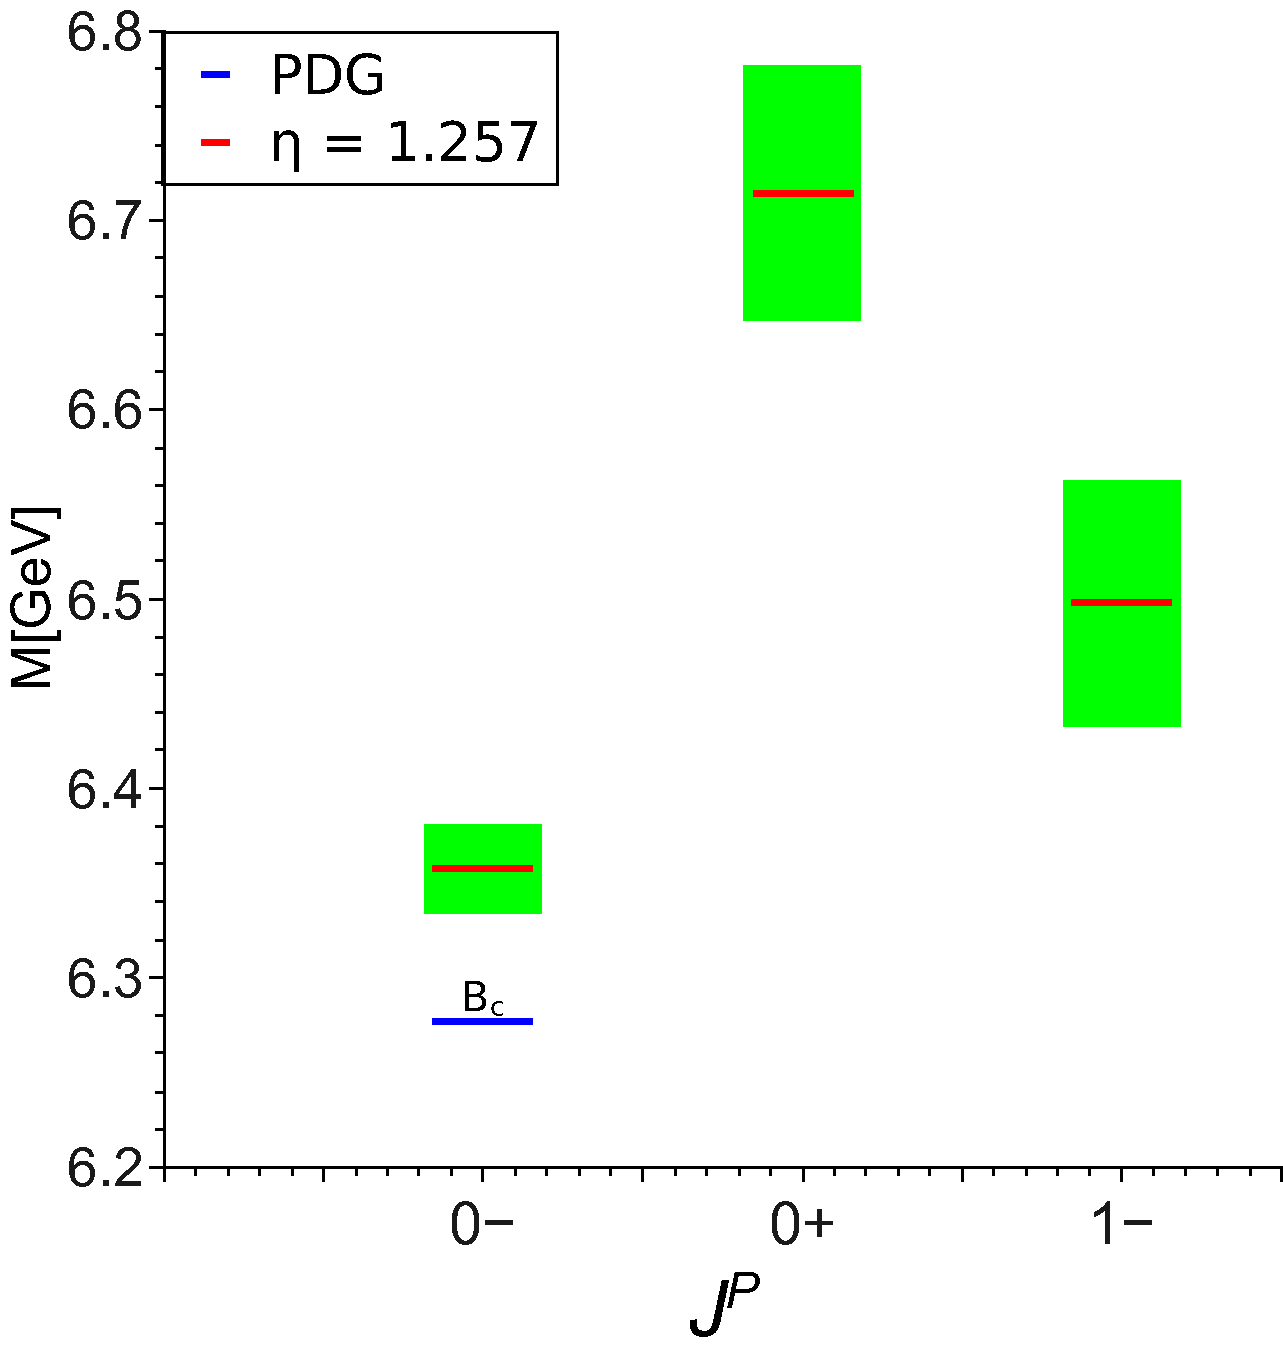
\includegraphics[width=0.45\textwidth]{figures/spectrum_bc}
    \caption{The calculated $b\bar{c}$ spectrum compared to experiment. The green bands correspond 
             to the variation $\eta=1.257\pm0.1$.}\label{fig:spectrumbc}
  \end{center}
\end{figure}
%
%
\begin{table*}[!t]
\renewcommand{\arraystretch}{1.3}
\begin{center}
\begin{tabular}{c|ccc|ccc||c|c}
\hline
\hline
            & \multicolumn{3}{c|}{$c\bar{c}   $}   & \multicolumn{3}{c||}{$b\bar{b}$}    & \multicolumn{2}{c}{$b\bar{c}$}                                         \\
$J^{PC}$    & $n=0$   & $n=1$  & $n=2$  & $n=0$   & $n=1$  & $n=2$  &  $J^{P}$ &    $n=0$                               \\
\hline                                                                                                                                                                                                     
$0^{-+}$    & $2925$  & $3684$ &        & $9414$  & $9987$ &    	&   $0^{+}$     &   $6714^{+67.1}_{-67.1}$           \\
$0^{--}$    & $3348$  &        &        & $9642$  &        &    	&   $0^{-}$   &     $6354^{+23.5}_{-23.5}$    \\
$0^{++}$    & $3323$  & $3833$ &        & $9815$  & $10254$&    	&  $1^{+}$   &                         \\
$0^{+-}$    & $3674$  &        &        & $10014$ &        &     	&  $1^{-}$  &     $6498^{+64.9}_{-64.9}$                                 \\
\hline                                                                                                                                                                                                     
$1^{-+}$    & $3524$  &        &        & $9788$  &        &    	&       &                 \\
$1^{--}$    & $3113$  & $3676$ & $3803$ & $9490$  & $10089$& $10327$&       &               \\ 
$1^{++}$    & $3489$  & $3672$ & $3912$ & $9842$  & $10120$& $10303$&       &               \\
$1^{+-}$    & $3433$  & $3747$ &        & $9806$  & $10154$&    	&       &                    \\
\hline                                                                                                                                                                                                     
$2^{-+}$    & $3806$  &        &        & $10194$  &        &    	&      &                                 \\
$2^{--}$    & $3739$  &        &        & $10145$  &        &    	&      &                                              \\
$2^{++}$    & $3550$  &        &        & $9906$   &        &    	&      &                                      \\
%$2^{+-}$   &         &        &        & $10194$  &        &    	&     &                                                                      \\
\hline                                                                                                                                                                                                     
%$3^{-+}$   &         &        &        &          &        &    	&      &                                        \\
$3^{--}$    & $3896$ &         &        & $10232$  &        &    	&      &                                           \\
$3^{++}$    & $3999$ &         &        & $10302$  &        &    	&       &                                     \\
$3^{+-}$    & $4037$ &         &        & $10319$  &        &    	&      &                                                   \\                                                                                                                                                                      
\hline
\hline
\end{tabular}
\caption{Calculated masses for ground and excited charmonium, bottomonium and charm-bottom states.}\label{tab:results_heavy}
\end{center}
\end{table*} \\

Finally, we present our results for selected channels of $B_c$-mesons. 
Heavy-light systems in the Bethe-Salpeter% PARTITIONING OPTIMIZATION \beware 
approach are notoriously difficult to treat, since the problem of probing the analytical
structure of the internal quark propagators already appears for ground states, see e.g.
Ref.~\cite{Rojas:2014aka,Gomez-Rocha:2014vsa} for recent studies of the problem. Our results for these states,
shown in Fig.~\ref{fig:spectrumbc} are therefore all extrapolated and have a systematic error
of about 5-10 \%. In the plot we show values obtained using a variation of the $\eta$-parameter
in the interaction ranging approximately between the ones used for the charmonia and bottomonia.
In this way we heuristically take into account the varying strength of the interaction for the
two different quark flavours involved. The central value, given by the red line, corresponds 
to $\eta=1.257$. Given the inherent uncertainties in the calculation, our value for the $B_c$
in the pseudoscalar channel is surprisingly close to the experimental one. Since this is the
state with the lowest mass, the extrapolation error is also smallest. Since the rainbow-ladder
approach works well in the vector channel we consider the existence and to some extent also the 
mass of the vector state as a prediction of the approach, whereas the scalar channel has to
be considered with much more reservation. Despite these sources for errors it is interesting to
note that our results for all three states agree qualitatively with the ones in the relativistic 
quark model of Ref.~\cite{Ebert:2011jc} with quantitative deviations of at most 3~\%.

\subsection*{Effective interaction variation}\label{int1}
As we saw, the interaction between heavy quarks, represented by effective singe gluon exchange, leads to 
the spectrum coinciding with experimental values with in 5\%. The main reason for that is the huge set of diagrams like: hadronic exchange, quark loops and etc. are suppressed by heavy quark mass. From this fact follows that the charmonium meson bound state is a prefect test-ground for a effective gluon models. Therefore it is interesting to explore the response of the mass spectrum to the variation of the shape of the effective gluon coupling $\alpha_{eff}$. In order to proceed with this idea we would like to replace the original Maris and Tandy model \cite{Maris:1999nt}, which explicit expression is:
\beqa
\label{spec:MT_model}
\alpha_{\mathrm{eff}}(q^2)=\pi\eta^7x^2e^{-\eta^2x}
+\frac{2\pi\gamma_m\left(1-e^{-y}\right)}{\log\left[e^2-1+(1+z)^2\right]}\;,
\eeqa
with more generalized form:
\begin{align}\label{spec:generalmaristandy}
%
  \alpha_{\mathrm{eff}}(q^2)=\alpha_{\mathrm{IR}}(q^2)+\alpha_{\mathrm{UV}}(q^2)\;,
%
\end{align}
%
where
%
\begin{align}\label{spec:generalmaristandy2}
%
  \alpha_{\mathrm{IR}}(q^2) &= \pi\eta^7\mathcal{P}(x)e^{-\eta^2x}\;,\\
  \alpha_{\mathrm{UV}}(q^2) &= \frac{2\pi\gamma_m\left(1-e^{-y}\right)}{\ln\left[e^2-1+(1+z)^2\right]}\;.
%
\end{align}
Since expect the shape of the interaction to change we therefore employ the polynomial form for $\mathcal{P}(x)$:
\begin{align}\label{spec:polinomMT}
%
  \mathcal{P}(x) = \sum_{i=1}^n a_i x^{i}\;.
%
\end{align}
%
and investigate its impact on the heavy meson spectrum restricting ourselves 
to terms with $n \le 4$. Note that $a_2=1$ and other $a_n=0$ corresponds to original Maris and Tandy model. 
\begin{figure}[!t]
  \begin{center}
    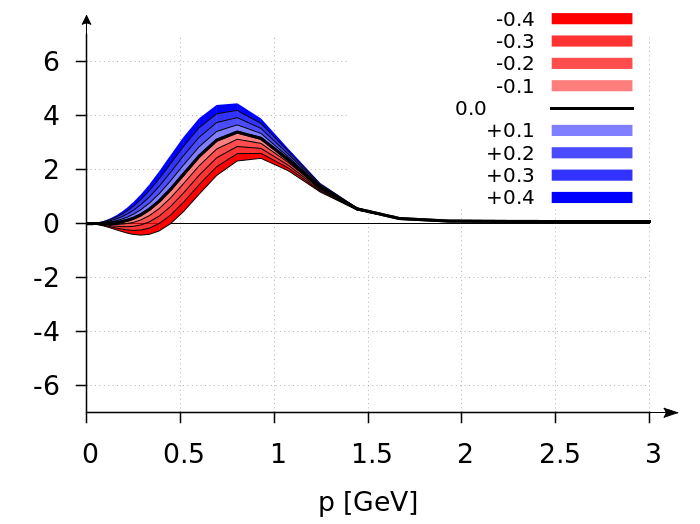
\includegraphics[width=0.49\textwidth]{figures/maris_a1}
    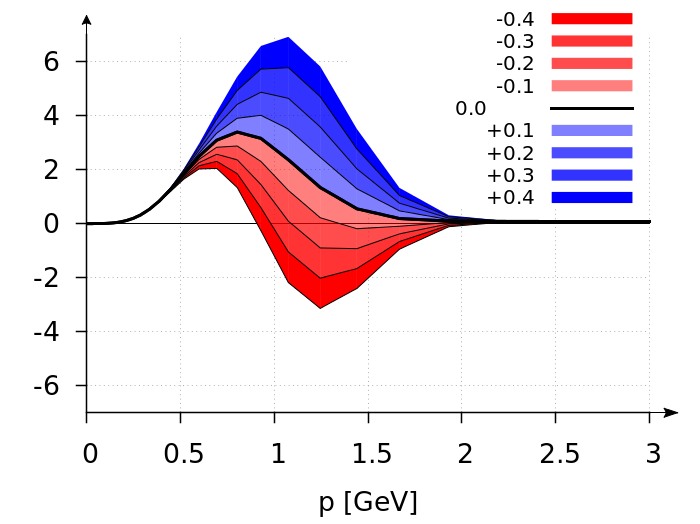
\includegraphics[width=0.49\textwidth]{figures/maris_a4}
    \caption{The shape of the effective coupling for the generalized Maris-Tandy interaction with $a_2=1$ held constant
             and varying $a_1$ and $a_4$. Left graph corresponds to the variation of $a_1$ and right one to the variation of $a_4$. }
    \label{fig:slope_a1}
  \end{center}
 \end{figure} \\
 
First we vary $a_1$ in the interval
$-0.5 \le a_1 \le 0.5$. For the effective running coupling the resulting variation
is shown in Fig.~(\ref{fig:slope_a1}). Clearly, the integrated strength, but
also the fine details of the coupling change: For negative $a_1$ we even obtain 
a zero crossing with the corresponding scale associated with the relative
strength between the $a_1$ and $a_2$-terms (here we keep $a_2=1$). Such an 
effective coupling is unusual, but not unreasonable. Recent calculations of 
the three-gluon vertex \cite{Aguilar:2013vaa,Blum:2014gna,Eichmann:2014xya} suggest that the interplay between 
ghost and gluon degrees of freedom in the corresponding Dyson-Schwinger equation 
for the vertex may very well introduce such a zero crossing. This possibility is also 
seen in corresponding lattice calculations \cite{Cucchieri:2008qm}. Since the three-gluon 
vertex is an integral part of the non-Abelian diagrams in the DSE for the quark-gluon vertex, 
this behaviour may translate into a corresponding zero crossing of the quark-gluon 
vertex~\cite{Williams:2014iea} and subsequently into the effective coupling.  
 \begin{figure}[!t]
  \begin{center}
    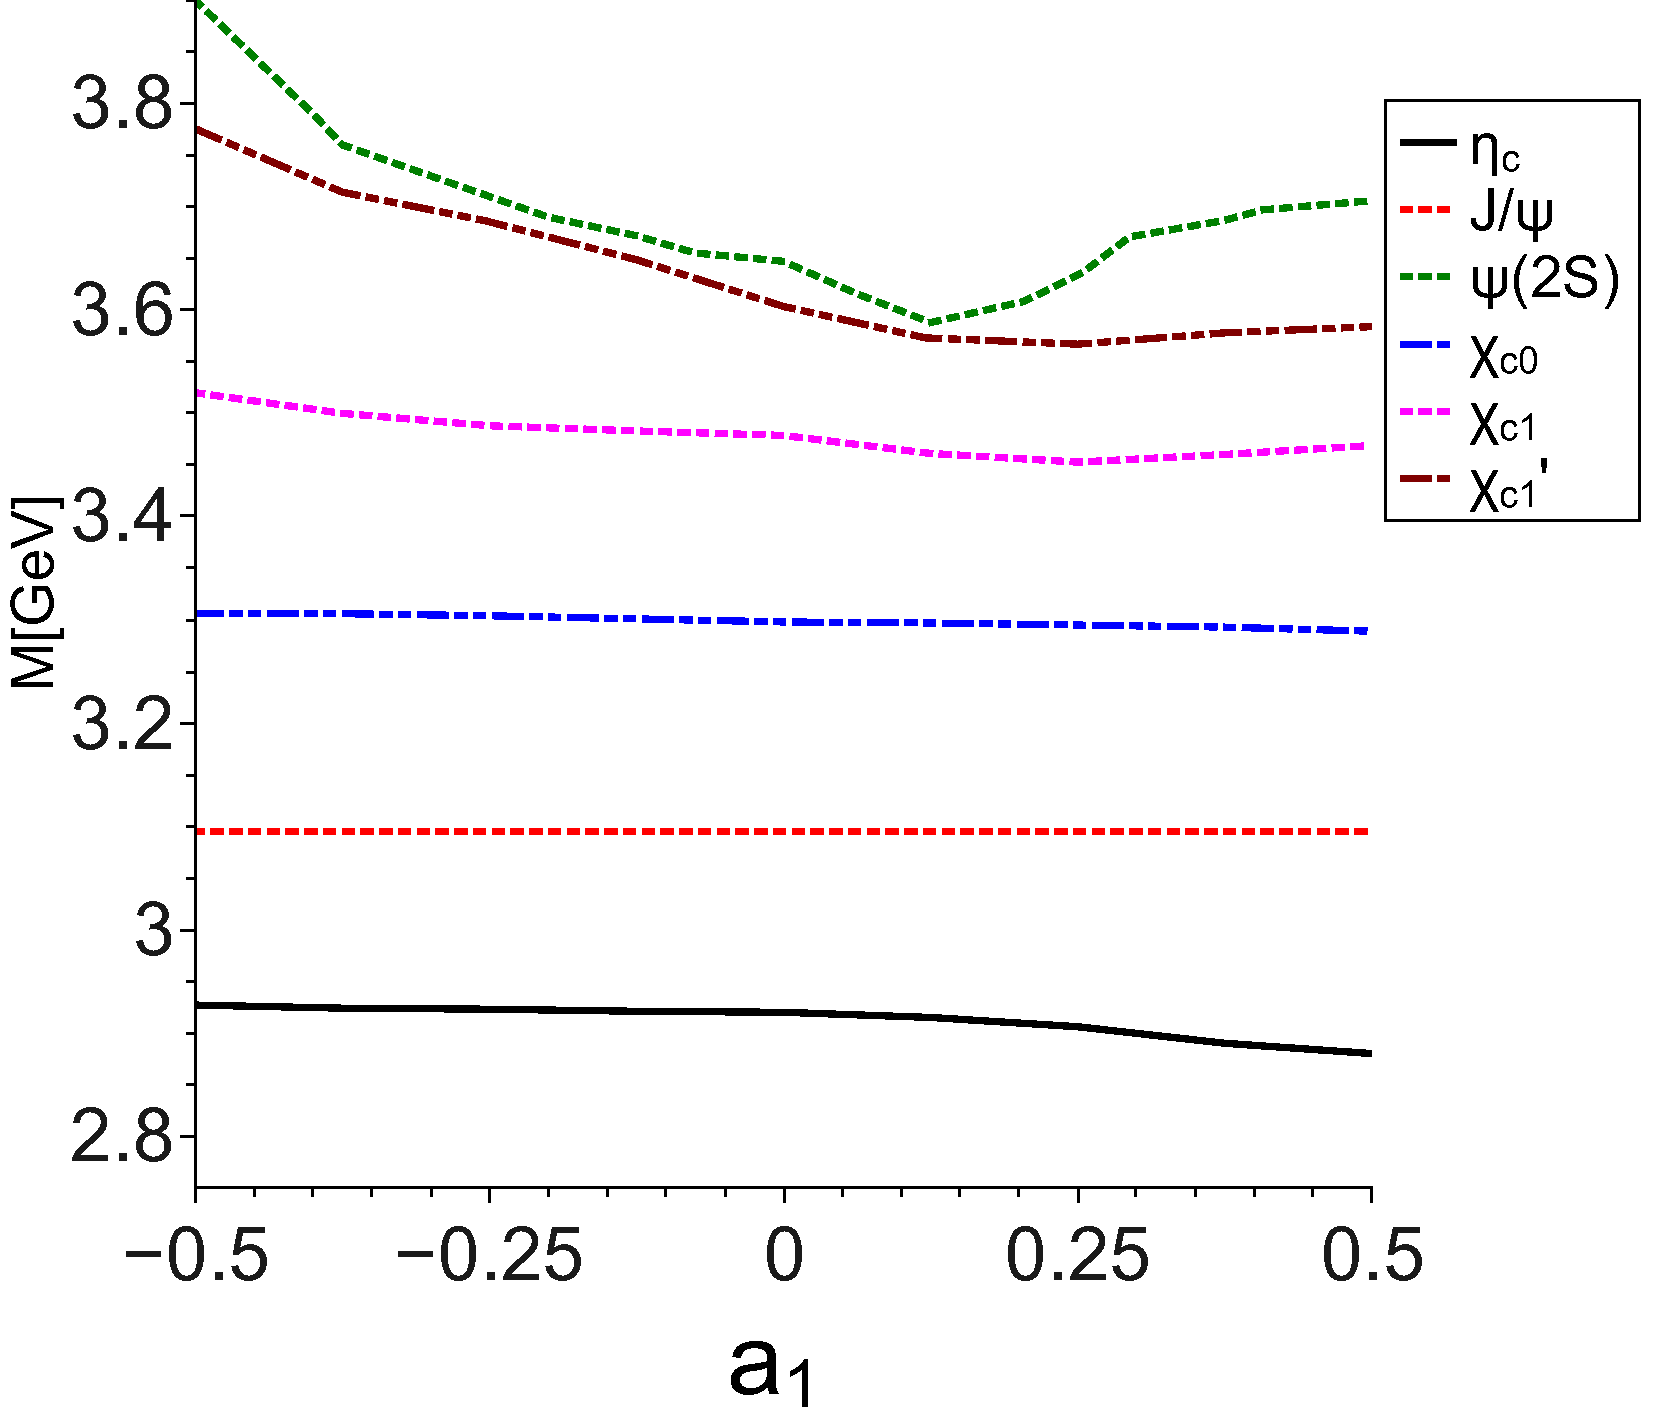
\includegraphics[width=0.49\textwidth]{figures/trend_a1_CC}
    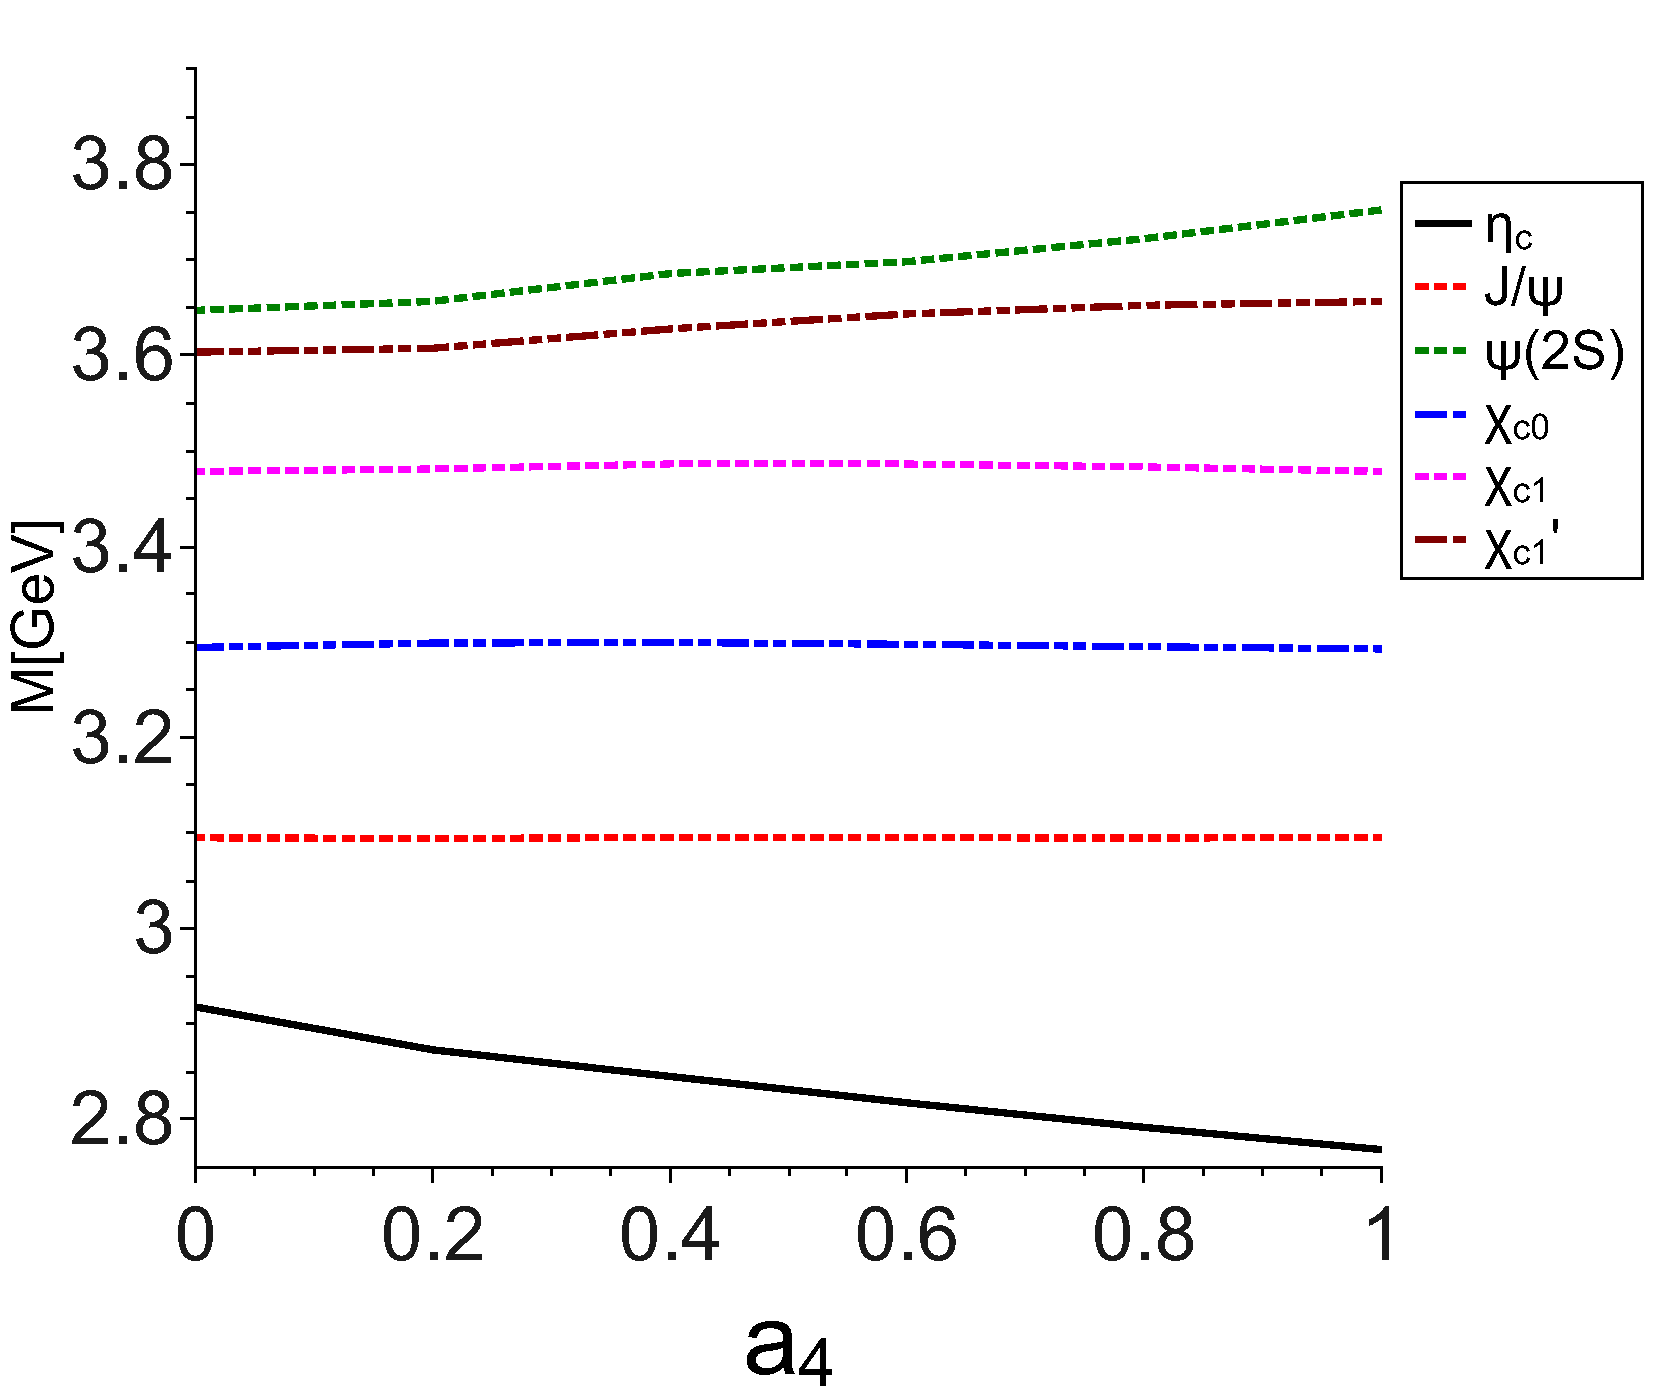
\includegraphics[width=0.49\textwidth]{figures/trend_a4_CC} 
    \caption{The response of masses of bound and excited states on the variation of the shape 
             of the effective interaction with $a_1$ and $a_4$ correspondingly.}
    \label{fig:trend_a1}
  \end{center}
\end{figure} \\

The resulting changes in the meson spectrum are displayed in 
Fig.~\ref{fig:trend_a1}. Adjusting the bare charmonium quark mass via $m_{J/\Psi}$
to accommodate for the changes in the integrated interaction strength we
observe only very small changes in the resulting masses for the ground state mesons.
However, the excited states $\Psi(2S)$ and $\chi_{c1}^{\prime}$ turn out to be very sensitive 
to the details of the interaction. In particular for negative values of $a_1$,
corresponding to the zero crossing of the interaction discussed above, we find much
increased values for the mass of the $\chi_{c1}^{\prime}$, which eventually even may 
hit the experimentally observed mass of the $X(3872)$. However, this comes at a price: 
the mass of the $\Psi(2S)$ reacts in a similar way and substantially moves away from 
the experimental value, almost reproduced for $a_1=0$. We therefore conclude, that 
by changing the infrared behaviour of our rainbow-ladder interaction it is not possible 
to accommodate for the quark-antiquark nature of the $X(3872)$, while at the same time 
keeping the remaining spectrum intact. \\

Next we consider the generalized Maris-Tandy interaction, Eq.~(\ref{spec:generalmaristandy2}), 
given by $a_1=0$, $a_2=1$ but non-trivial components $a_3$ or $a_4$. Both of these modify 
the interaction in the intermediate momentum region, while keeping the infrared and
ultraviolet behaviour untouched as can be seen from Fig.~\ref{fig:slope_a1} for the 
example of variations in $a_4$. Since variations of $a_3$ act similarly on the effective
coupling we keep $a_3=0$ fixed and restrict ourselves to variations of $a_4$.
Furthermore, we keep $a_4 \ge 0$, since there are no indications that the dressing of the
quark-gluon vertex can induce a negative effective interaction in the mid-momentum region. \\

Again, we study the variation of the charmonium spectrum while still readjusting
the charm quark mass to reproduce the vector ground state $J/\Psi$. Our results
are given in Fig.~\ref{fig:trend_a1}. Here we find a substantial increase in the
mass splitting between the pseudoscalar and the vector channel due to the additional
interaction strength in the mid-momentum region. At the same time, the masses of the
excited state, $\Psi(2S)$ and $\chi_{c1}^{\prime}$ increase slightly. This moderate increase 
is nowhere large enough to bring the $\chi_{c1}^{\prime}$ close to the observed $X(3872)$-state.
Thus we arrive at the conclusion that by changing the mid-momentum behaviour of our 
interaction it is not possible to accommodate for a quark-antiquark nature of the 
$X(3872)$, while at the same time keeping the remaining spectrum intact.
%
%
%
%

\section{Regge trajectories}\label{res:regge}
Finally, we present results for Regge trajectories in Fig.~\ref{fig:regge} for natural parity states. 
At first, we consider the ground states of the light quark meson spectra; for the corresponding excited states and the 
other channels we do not have enough bound states with $J=2,3$ to probe for trajectories. 
One immediately notes that, indeed, the sequence $J^{PC}=1^{--}, 2^{++}, 3^{--}$ forms an almost linear
trajectory in the $(M^2,J)$-plane. This is interesting, since we are working with a model that is
apparently \emph{not} related to a linear rising potential between light quarks. 
\begin{figure}[h]
\begin{center}
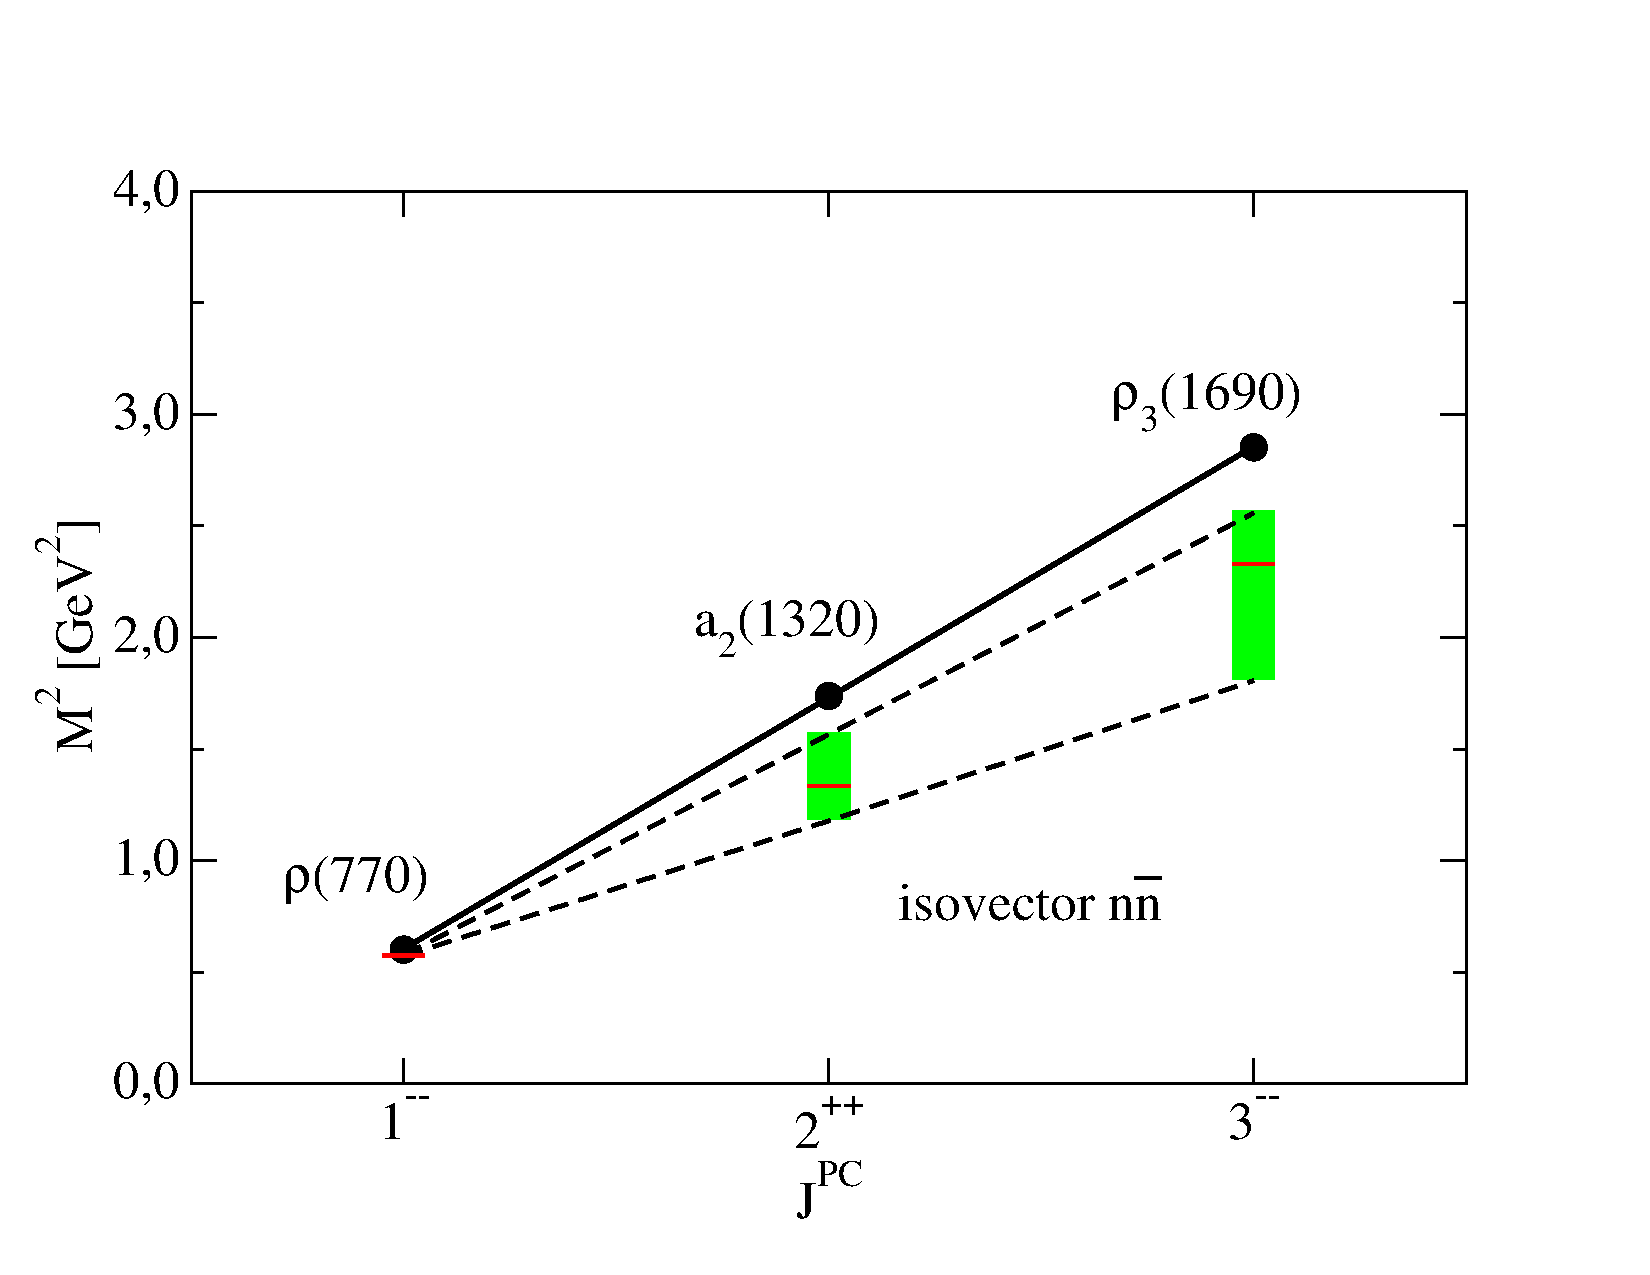
\includegraphics[width=0.49\textwidth]{figures/reggenn_v2}
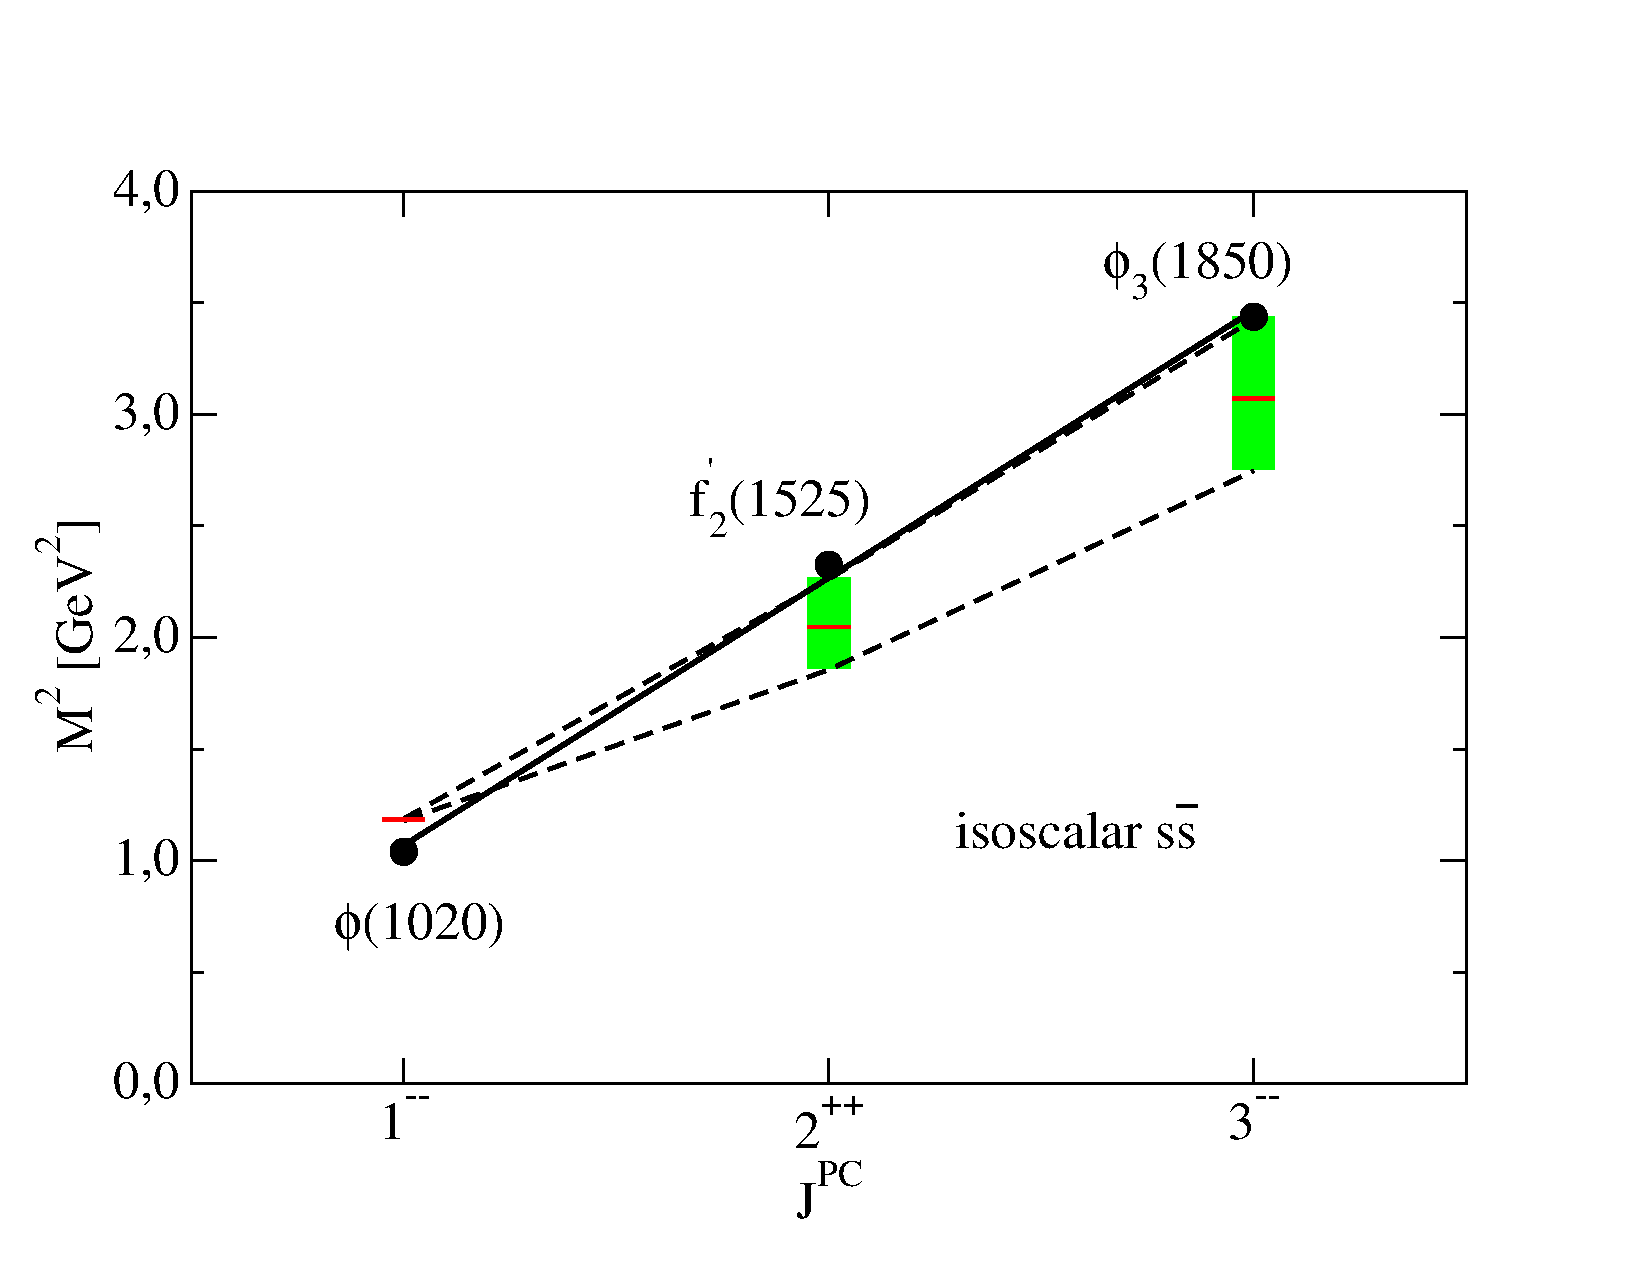
\includegraphics[width=0.49\textwidth]{figures/reggess_v2}
\caption{\small Regge trajectories for isovector $n\bar{n}$ (upper plot)
and isoscalar $s\bar{s}$ mesons (lower plot) with natural parity. 
Filled circles correspond to experimental data, while calculated values are given by the red marks
for $\eta = 1.8$ and the green bands for $\eta = 1.8 \pm 0.2$. The resulting Regge trajectories for 
the upper and lower end of the bands are displayed by the dashed lines. Not shown is the numerical
error of our mass extraction procedure, which is of the order of 5-10 $\%$ for the $J=2,3$ states.}\label{fig:regge}
\end{center}
\end{figure} 
Thus, the conventional, naive but intuitive explanation for the formation of Regge-trajectories does not apply
in our framework. Nevertheless, we see an (approximate) $\rho$- and $\phi$-meson Regge trajectory 
for our results. The slope of the trajectory is easily extracted. With
\begin{equation}
M^2_X(J) = M^2_X(0) + \beta_X J
\end{equation} 
we find
\beqa
M^2_\rho(0)& = -0.42 \,\,(-0.05)\,\, \mbox{GeV}^2 \;\;\;\;  M^2_\phi(0)& = \,\,0.05 \,\,(0.36)\,\, \mbox{GeV}^2 \nonumber\\
\beta_\rho & = \,\,0.99 \,\,(0.62)\,\, \mbox{GeV}^2  \;\;\;\;\;\;\;\;\;\;\;\;\;\;\; \beta_\phi &  = \,\,1.12 \,\,(0.78)\,\, \mbox{GeV}^2 \nonumber
\eeqa
for $\rho$ and $\phi$ respectively. The two numbers each correspond to the upper (lower)
end of the $\eta$-band of our results. Compared to recent studies of Regge trajectories
based on the $\rho$-meson, $\beta_\rho = 1.19 \pm 0.10$ GeV$^2$ \cite{Masjuan:2012gc} and 
$\beta_\rho = 1.11 \pm 0.01$ GeV$^2$ \cite{Londergan:2013dza}, our number for the slope at the
upper edge of the $\eta$-band is smaller by only about 
ten percent. Recalling that we need to employ an extrapolation procedure in the complex 
momentum plane to extract the bound state mass of the tensor states with an error margin 
of the order of 5-10 $\%$ the agreement is quite good.
We have also checked for Regge trajectories in channels with unnatural parity and found an 
approximate linear trajectory also for the sequence $J^{PC}=1^{++}, 2^{--}, 3^{++}$ based 
on the $a_0$. Again, for the other channels and the excited states we find not enough bound 
states with $J=2,3$. From the discussion in the previous sections we furthermore expect, 
that the slopes and intercepts in these channels may be further off the experimentally extracted 
values, simply because the rainbow-ladder interaction is not good enough in these channels. 
Indeed for the $a_0$-trajectory we find $M^2_{a_0}(0) = 0.20\,\, \mbox{GeV}^2$ and
$\beta_{a_0} = 0.78 \,\,\mbox{GeV}^2$ for the upper edge of the $\eta$-band, which do not 
agree too well with {\it e.g.} the values found in Ref.~\cite{Ebert:2009ub}, 
$M^2_{a_0}(0) = -0.658 \pm 0.120\,\, \mbox{GeV}^2$ and
$\beta_{a_0} = 1.014 \pm 0.036 \,\,\mbox{GeV}^2$. \\

As for the heavy quark systems, similar to the light quark sector we also find, that the 
sequence $1^{--}, 2^{++}, 3^{--}$ lies on a Regge-trajectory with an accuracy that is
even better than in the potential model of Ref.~\cite{Ebert:2011jc}. 
For $M^2_X(J) = M^2_X(0) + \beta_X J$ we find $M^2_{J/\psi}(0) = 2.72$ and $\beta_{J/\psi} = 0.39$ for charmonium natural parity states and
for bottomonium - $M^2_{\Upsilon}(0) = 9.12$ and $\beta_{\Upsilon} = 0.371$, which 
is also somewhat steeper than the result of \cite{Ebert:2011jc}. For the heavy quark 
sector this confirms a result for light quarks, that Regge-type behaviour in the spectrum may be 
found without any direct connection to an underlying string-picture.
%
%
%
%
%
%In this work we presented a first calculation of ground and excited states with angular 
%momentum $J \le 3$ in the heavy quark sector using the framework of Dyson-Schwinger 
%and Bethe-Salpeter equations. We have used a simple interaction model, the rainbow-ladder
%approximation, which is known to represent only part of the complicated interaction
%pattern of quarks and gluons even for heavy quarks. Nevertheless, we obtained surprisingly 
%good results, at least for selected quantum numbers. In general, the systematics in the 
%spectrum for charmonia and bottomonia is very similar, although the underlying interaction 
%is not the same. Compared to the light quark sector, where
%the rainbow-ladder approximation has clear deficiencies \cite{Fischer:2014xha}, the agreement with
%the experimental states is much improved. This is particularly true for the ground and 
%excited charmonia and bottomonia states in the vector channel, where even the second 
%radial excitation is well represented. For pseudoscalar states and tensor states with quantum 
%number $2^{++}$ we obtain reasonable results, whereas for scalars and axialvectors some
%deviations occur. We also gave predictions for the other tensor states, in particular
%for the $3^{--}$, which should be a channel where the rainbow-ladder approximation
%does particularly well. For the bottomonia, our values for the tensor states may be 
%considered as solid predictions for experiment with a systematic error due to 
%extrapolations on the 1~\% level. We also gave results for $B_c$ states and quarkonia 
%with exotic quantum numbers, although the accumulated errors in these channels due to
%deficiencies in the rainbow-ladder interaction may be sizeable.
%
%Furthermore, we studied variations of the shape of the rainbow-ladder effective coupling with 
%the aim to explore whether the first excitation in the $1^{++}$-channel can be linked 
%to the $X(3872)$ without destroying other parts of the spectrum. It turned out, that 
%this is not possible. Thus either hitherto not included corrections beyond rainbow-ladder
%play an important role in this channel, or the $X(3872)$ does indeed not have a strong
%quark-antiquark component. From the perspective of our framework, these questions remain 
%open until studies beyond rainbow-ladder are available. 
%
%Clearly, the findings of this work should be corroborated by studies beyond the 
%simple rainbow-ladder scheme used in this work. Within the light meson sector
%several approaches in this direction have been explored in the past 
%\cite{Watson:2004kd,Fischer:2005en,Fischer:2008wy,Fischer:2009jm,Chang:2009zb,Heupel:2014ina}
%and it remains to be seen whether these can be transferred to the heavy quark 
%sector. This will the subject of future work.
	


